\documentclass[12pt, oneside]{book}
%\documentclass[12pt]{book}

\usepackage{ circuitikz }
\usepackage{graphicx} % Required for inserting images
\usepackage{subcaption}
\usepackage{tabularx}
\usepackage{algorithm}
\usepackage{algpseudocode}

\usepackage{svg}
\usepackage{listings}
\usepackage{parskip}
\usepackage{dcolumn}% Align table columns on decimal point
\usepackage{xcolor}
\usepackage{bm}% bold math
\usepackage{mathrsfs}
\usepackage{amsfonts, amsthm, amsmath, amssymb}
\usepackage{svg}
% Tikz diagrams/schematics
\usepackage{tikz}
\usepackage{siunitx}

\usetikzlibrary{calc, shapes.geometric, arrows.meta, positioning}
%bibliography


\usepackage{microtype} % Subtle font spacing adjustments
\usepackage
[
        a4paper,% other options: a3paper, a5paper, etc
        left=0.75in,
        right=0.75in,
        top=1in,
        bottom=1in
        % use vmargin=2cm to make vertical margins equal to 2cm.
        % us  hmargin=3cm to make horizontal margins equal to 3cm.
        % use margin=3cm to make all margins  equal to 3cm.
]
{geometry}

\usepackage{setspace}
\onehalfspacing % Or \doublespacing for thesis-level spacing

\usepackage{biblatex}
\addbibresource{references.bib}

\usepackage{nomencl}
\makenomenclature
\renewcommand{\nomname}{List of Symbols}
\renewcommand{\nompreamble}{The next list describes several symbols that will be later used within the body of the document}

\newtheorem{theorem}{Theorem}
\newtheorem{definition}{Definition}
\newcommand{\sbracket}[1]{\left[ #1\right]}
\newcommand{\bracket}[1]{\left( #1\right)}
\newcommand{\R}{\mathbb{R}}

\newcommand{\ipw}[2]{\left\langle #1,\, #2 \right\rangle_w}


\begin{document}

    \begin{titlepage}
        \begin{center}

        % University name
        {\Large\textbf{THE UNIVERSITY OF BRITISH COLUMBIA}}\\[2cm]

        % Thesis title
        {\Large \bfseries CONFINED DIFFUSION OF NANOPARTICLES USING iSCAT MICROSCOPY}\\[2cm]


        % Author
        by\\[0.5cm]
        {\Large Martin Jasinski}\\[2cm]

        % Submission line
        A THESIS SUBMITTED IN PARTIAL FULFILLMENT OF\\
        THE REQUIREMENTS FOR THE DEGREE OF\\[0.5cm]

        % Degree type
        {\Large Master of Applied Science}\\[0.5cm]

        % Program
        in\\[0.5cm]
        {\Large (Engineering Physics)}\\[0.5cm]

        % Institution
        {\Large THE UNIVERSITY OF BRITISH COLUMBIA}\\[0.5cm]

        % Campus (if applicable)
        {\Large Department of Physics}\\[1cm]

        % Date (month and year only)
        {\Large \today}

        \vfill

        \end{center}
    \end{titlepage}
    

    \section*{Layman Summary}

%MARTIN GOOD
% Many products are made using very tiny pieces of material called nanoparticles. These are found in things like plastics, medicines, and food. To make sure these products are safe and good quality, we need to measure what these tiny pieces are like. For example, their size and how they behave.

% However, nanoparticles are so small that we cannot see them clearly, even with a microscope that uses light. So we need to find new ways to study them.

% This thesis develops an alternative method to do this. It measures where a particle is located in space, and it watches how that position changes over time. Using mathematics, we can then learn more about the particle from the way it moves. This helps us measure nanoparticles more accurately.

% CRINGE
The thermal motion of particles has been extensively studied to understand the influence of temperature on particle interactions. Thermal behavior is typically characterized by the temperature of a body or environment, which represents the average kinetic energy of a large ensemble of particles and follows the Maxwell–Boltzmann statistical distribution. However, the influence of temperature on the behavior of individual particles within a complex environment remains less understood.

A more detailed understanding of thermal motion at the single-particle level requires the ability to observe and analyze the trajectories of individual particles. Single-particle tracking (SPT) provides this capability through particle labeling, high-resolution imaging, and computational trajectory reconstruction, enabling direct measurement of particle dynamics with high spatial and temporal resolution.

This thesis presents a method for three-dimensional single-particle tracking using interferometric microscopy. The proposed approach enables precise localization of individual particles in three dimensions and reconstructs their trajectories over time.

Analysis of the reconstructed trajectories allows the extraction of important physical parameters, including the mean squared displacement (MSD), diffusion coefficient, drift velocity, interaction forces, particle size, and confinement effects. These measurements provide quantitative insight into the thermal motion and interactions of individual particles, offering a powerful tool for investigating nanoscale processes that cannot be resolved through ensemble-averaged measurements alone.


%better
% In scientific manufacturing, such as plastics, pharmacology, and food science small molecules, known as nano-particles, are part of the product or procedure. In order to ensure that the output product is of high-quality or up to standard, one tends to want to measure the properties of these nanoparticles. However, due to their size being smaller than that resolvable by light alone, there is a need to develop new methods to do this. This thesis aims to develop one such method to measure three-dimensional particle position in space, and mathematically extract information from this position in time to better improve measurements of nanoparticle characteristics.

% intro
%Particle confinement allows for extended measurements of suspended biomolecules and nanoparticles using optical microscopy as it keeps it within the field of view.

\newpage
\section*{Abstract}
The understanding of thermal movement of paricles within a confined space has been studied extensively in order to understand biological, chemical, and physical processes. Although the theoretical understanding of this confined diffusion is well defined in literature, not much work has been done to understand the effects of electrostatic and hydrodynamic contributions to the size measurements measured from the motion of nanoparticles, as measurements are often intrinsically performed under confinement. This is due to the fact that 3D particle-tracking is not as commonly used as other, higher throughput sizing techniques. By employing developed techniques of nanoparticle tracking in tandem with a full theoretical model, the non-trivial effects of confinement on size-diffusivity were directly investigated and characterized. The work described in the thesis advances the method and tools of 3D nanoparticle analysis both theoretically and in application.

% This thesis provides an understanding and investigation into confined diffusion measurements.

The first section of the thesis describes a theoretical model of Brownian motion based on the confined-Langevin model using a Debye-Hückel electrostatic potential. The model was implemented, based on literature \cite{millanNumericalSimulationsConfined2023}, into a computer-based Python simulation in order to parameterize and create prior distributions of particle motion. 

The second section describes a modified method of 3D tracking to obtain faster calculations of particle position from optical microscopy images. This was based on an algorithm described in literature \cite{dewitPreciseCharacterizationNanometerscale2023}. The validation of the method was done on exact point-spread function simulation data with an accuracy of 1 nm.  

The third section describes the acquisition of  experimental data using a custom interferometric scattering microscope (iSCAT) with image pixel resolution 55 nm acquiring images between 400 and 1000 frames per second. The data consisted of images of scattering fringes from nanoparticle species and was analyzed using the algorithm developed in section 2. The resultant information was accurate 3D particle tracks. The models developed in section 1 were applied to the tracks to obtain infer particle size and charge. 

The thesis presents a method of finding particle size, motion, and electrostatics which can present additional tools to analyze nanoparticle characterization, which was the goal of the thesis. 

\section*{Acknowledgements}

I would like to thank for the guidance, help and resources from Dr. Sabrina R. Leslie, who is also my supervisor of thesis. In addition, I would like to thank Dr. Erik Olsén, a post-doc in the Leslie-Lab, who collaborated and provided guidance to me during this project.

    \tableofcontents
    
    % list of symbols
    \nomenclature{\(\delta_{ij}\)}{Kronecker's delta function}
    \nomenclature{\(\delta(\cdot)\)}{Dirac's delta function}
    \nomenclature{\(\vec{x}\)}{Position Vector}
 	
	\nomenclature{\(\vec{v}\)}{Velocity Vector}
	\nomenclature{\(m\)}{mass}
	
	\nomenclature{\(t\)}{time}
	\nomenclature{\(\kappa\)}{Inverse of Debye-length}
	\nomenclature{\(\zeta_p\)}{particle zeta-potential}
	\nomenclature{\(\psi_w\)}{wall zeta-potential}
	\nomenclature{\(\Gamma_i\)}{Stern Layer of species \(i\)}
	\nomenclature{\(\Gamma\)}{Fluctuation-dissipation magnitude}
	\nomenclature{\(j\)}{Probability current}
	\nomenclature{\(W_t\)}{Gaussian white noise process}
	\nomenclature{\(\sigma_w\)}{Surface charge density}
    \nomenclature{\(D\)}{Diffusion coefficient}
	\nomenclature{\(h\)}{length}
	\nomenclature{\(\Psi\)}{Electrostatic potential}
	\nomenclature{\(\rho\)}{volumtric charge density}
	\nomenclature{\(\varepsilon_0\)}{permitivity of free space}
	\nomenclature{\(\varepsilon_r\)}{permitivity of material}
    \nomenclature{\(Z\)}{Ion number}
    \nomenclature{\(C\)}{Concentration}
    \nomenclature{\(\beta\)}{\(1/k_bT\)}
    \nomenclature{\(e_0\)}{Charge of an electron}
    \nomenclature{\(a\)}{Spherical particle radius}
    \nomenclature{\(\eta\)}{Fluid viscosity}
    \nomenclature{\(k_b\)}{Boltzmann Constant}
    \nomenclature{\(T\)}{Temperature}
    \nomenclature{\(\mu_\parallel\)}{Transverse mobility coefficient}
    \nomenclature{\(\mu_\perp\)}{Axial mobility coefficient}


    \printnomenclature
    
    % start document
    \chapter{Introduction}
    %\section{Motivation}

% - What is the major field i am in?
% - what are the biological questions 
% - how are they typically slved

% - problems with the current solutions


% In much of nature, the idea of size scales is widely discussed and investigated. From a basic understanding of physics, one understands that the forces an object feels are directly linked to their mass or volume and mass density. For example, we can easily understand what will happen to a basketball if we throw it up into the air as we are sitting on planet earth. However, when we leave the familar size scale, such as having a basketball the size of planet earth, or the size of a gas molecule, our intuition begins to show its cracks. 

Objects that exist in nature can be divided into macroscopic and microscopic entities. Macroscopic objects can be directly measured with a ruler or a photograph. However, as microscopic objects become smaller than the wavelength of light, they become un-resolveable by the light alone. Thus, one must resort to other methods to recover their size. 

At the nanoscale, thermal energy, $k_bT$, is comparable to, or larger than the gravitational and inertial energy scales that typical govern macroscopic dynamics. In the case of liquids, the thermal energy emerges into a motion in Reynold's numbers $\Re \ll 1$, where the viscous drag dominates ver the inertia. The result is a stochastic, thermal motion that governs particle transport. 

The relation between the particle's size and its motion is explained in Einstein's seminal paper \cite{einstein1956investigations} where the rate of transport, or diffusion is related to the particle's size,
\begin{equation}
    D(\vec{x}, a) = \frac{k_bT}{\gamma(\vec{x}, a)},
\end{equation}

where $\gamma(\vec{x}, a)$ is the viscous drag at the position $\vec{x}$ of a particle of hydrodynamic radius $a$. In the case of a spherical paricle in an incompressible fluid, $\gamma(a) = 6\pi \eta a$, where $\eta$ is the fluid viscosity. 

In typical measurements of particle motion, it is easiest to work in a confined space. For instance, convex-lens induced confinement (CLiC) measurements typically use micro-apertures of volume $\SI{1.5}{\micro \meter^3}$ to confine single molecules for extended temporal measurements via fluorescence microscopy. This is similar in the case of nanoparticle tracking analysis (NTA) measurements, where a flow is applied to particles confined between two plates in a flow-cell and are imaged using scattering microscopy. The confinement is performed as microscope images consist of 2D slices of a focal plane, which is typically on the order of a few hundred nanometers (cite). 

Although experimentally easier, the viscous drag relation is spatially varying. In turn, size-diffusivity relation in confinement is intrinsically non-trivial. This non-trivial behavior can been shown to alter the diffusivity of a particle by a significant amount \cite{swanParticleMotionParallel2010,bian111YearsBrownian2016}. 

Since the diffusivity of a particle in confinement is spatially varying, in order to recover the true size of a particle diffusing, it is necessary to have the full spatial location of the particle's motion with respect to the confinement barriers. This requirement necessitates the 3D tracking in confinement experiments. If one does not have the 3 dimensional position, one cannot recover the true size estimate.

In addition, one would like to view the molecules for enough frames to collect enough positional information to extrapolate the size. Thus, it would be better to use scattering microscopy over fluorescence as the photobleaching time of fluorescence and SNR is a hinderance to having quality data. 

\begin{figure}[ht]
    \centering
    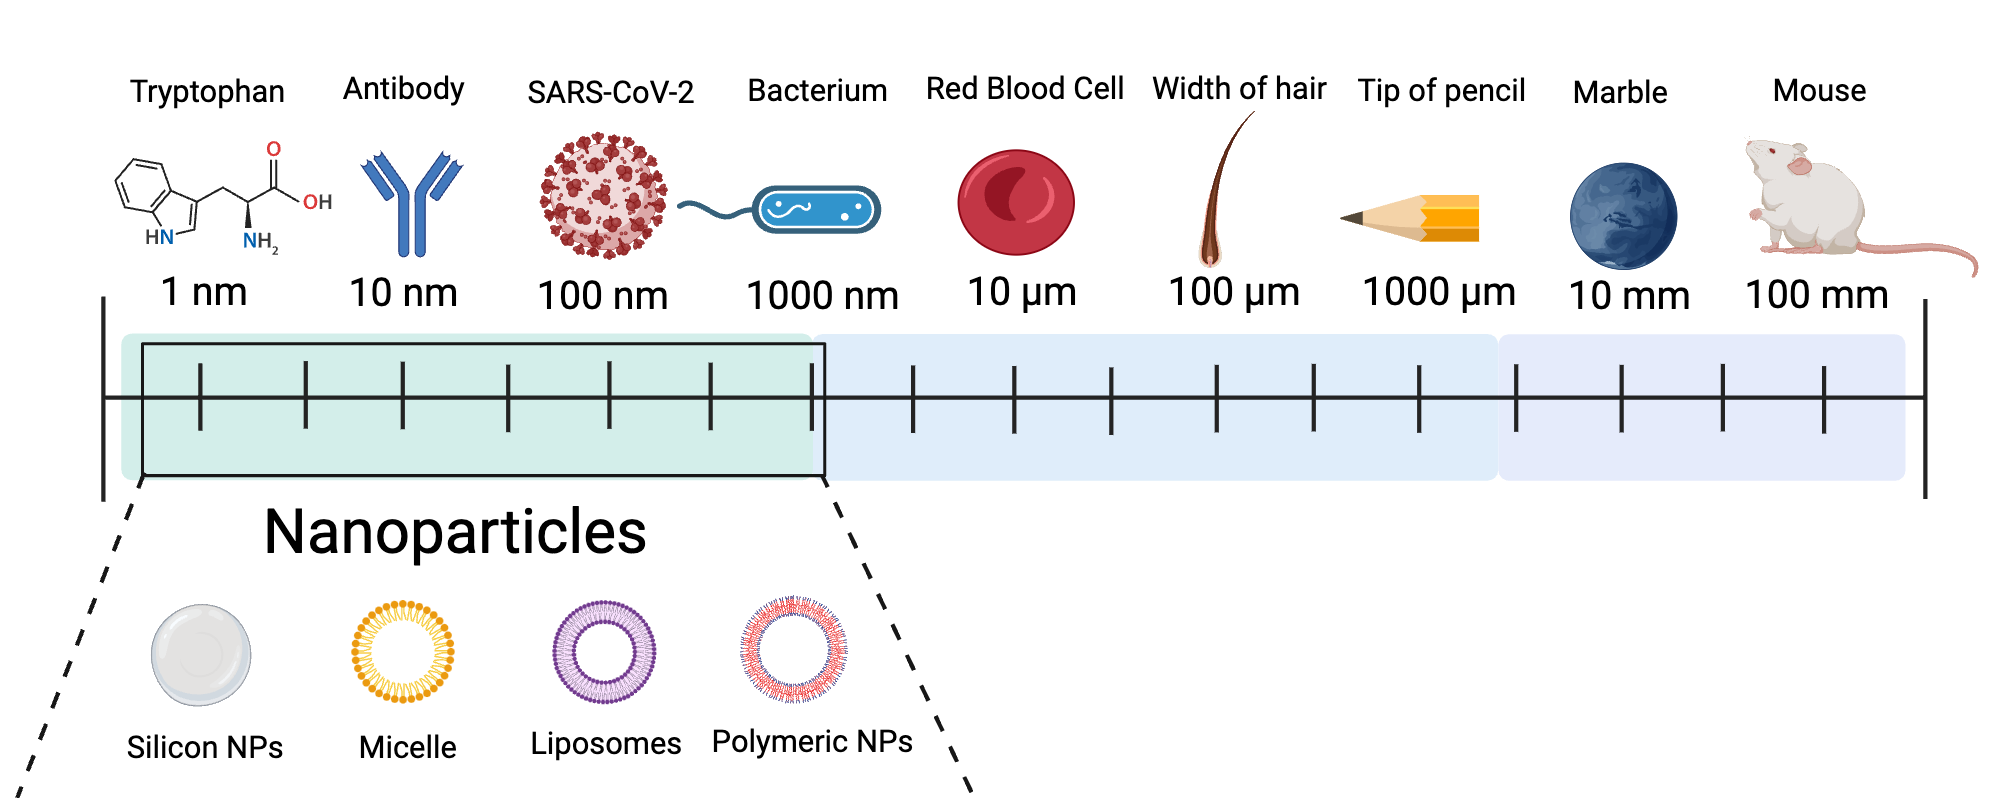
\includegraphics[width=\textwidth]{Figures/size-comp.png}
    \caption{Size comparison of various nanoparticles. Nanoparticles are defined as particles where the largest dimension is at most $\SI{1000}{\nm}$.}
\end{figure}

In the realm of biological processes, there are many such examples involving the particles in the nano size regime. For example, viruses and vesicles are two examples of small molecules which have immense importance in the field. To investigate such systems, it is often the case that to maintain long measurements of the same particle, it is necessary to have some form of confinement. The full understanding of the behavior of these nanoparticles under confinement is thus important, and not complete. 

The thesis consists of 8 chapters. Chapter 2 provides a description of the literature of confined brownian motion over the last century. Chapter 3 describes the theoretical description of interferometric scattering microscopy (iSCAT) and physical limits that apply in optical theory. Chapter 4 discusses the application of Brownian motion and iSCAT in a biological context, which details regarding lipid-nanoparticles and why they need to be studied on the single-molecule level. Chapter 5 consists of investigations of confined diffusion using Langevin simulations. A simulated system was developed and the size-diffusivity relation in an electrostatically screened system was investigated. Chapter 6 describes the 3D iSCAT tracking technique developed during this work. The method overview and validation and explicitly developed and validated Chapter 7 describes the method applied to experimental data and utilizes various nanoparticle species, highlighting their varied diffusions. Chapter 8 concludes the world and provides a future outlook on the topic and steps which need to be advanced.





    %\chapter{SPT in confinement principles }
    \iffalse
This section has the framework

1. Theory of the Molecular Dynamics 
2. Optical Physics and How we get signal (iSCAT)
3. Biological Applications 

Appendix 1.
- Basic E and M
- Charged surface potentials
- Stern Layers, Poisson Boltzmann ( Very short )
- Rayleigh Scattering Derivation (?)

Appendix 2
- Stochastic Processes
- Stationary solutions to the Smoluchowski Equation (Boltzmann Distribution)

Appendix 3.
- Fitting Methods used here
- L-BGFS

Appendix 4.
- Grid Traversal Algorithm
- Grid Search Method (?)
\fi

Biology is mostly nanoparticles. Nanoparticles move around stochastically under the rules of brownian motion. To be able to measure the particle's characteristics, one can relate their motion and stochasticity to their properties. This chapter will discuss the phenomena of Brownian motion and how it relates to particle properties, environmental ion concentration, viscosity, hydrodynamic boundaries, and confinement. To directly measure particle position, one can use optical methods, specifically, optical scattering measurements. In this chapter, the theoretical background regarding the particle's stochastic motion is presented, with particular focus on how the processes evolve in confined geometries. There will be a discussion on relating optical signals to their motion, as well as optical methods for particle detection. 




Methods that are able to detect single nanoparticles are known as single-molecule measurements. In the field of optical microscopy, single-molecule methods are often referred to as single particle tracking (SPT). This chapter aims to direct the reader through the theoretical context of the work done. First, Brownian motion is discussed, then optical preliminaries for SPT, and lastly, biological motivation is touched upon to continue the introductory words.



\section{Brownian Motion}
\iffalse
- Introduce the concept of Brownian Motion
- Histroy of brownian Motion
- applications of simple

- discuss an outlook of what has been done since then
- outline of this section
\fi

The physical phenomenon of diffusion can be rigorously described as the emergent behavior atomic particle undergoing random collisions with members of the surrounding environment. In the microscopic limit, where the radius of a particle is sufficiently small and thermal fluctuations dominate its dynamics, this erratic motion is referred to as Brownian motion \cite{brown_xxvii_1828}. 

\subsection{Classical Description of Einstein's Brownian Motion}

The classical description of Brownian motion is concerned with how the molecuar-kinetic theory of heat reates with microscopically visible size suspensions in liquid perform movements such that they can be viewed by a microscope. 


\subsection{Langevin Dynamics}

- Brownian motion can alternatively be described using a Langevin Model. 
- introduce langevin equation
- velocity correlation
- Arrive at the Fluc-Dissipation
- relate it to Einstein's formulation and show that given a stokes drag (sphere)

\begin{equation}
    D = \frac{k_bT}{\gamma_0}
\end{equation}

\subsection{Smoluchowski Equation}

- Since Langevin is kind of convient, how do we acctualy link the two methods?

- Fokker plank introdution motivated from the master equation
- - ideally summarize van kampen. 

- arrive at the general Smoluchowski equation for a random walker
- simple plots for descriptive purposes.

\section{Confined Diffusion Processes}

Although diffusion is interesting, there is a wealth of complexity in confinement due to Hydrodynamic effects
- quote 111 years here

- outline of this seciton

\subsection{Hydrodynamic Confinement}
- confinemnt from Hydrodynamics
- frictional slowing
- ...

\subsection{Geometric Confinement}
- i need to check references on if this is relate

\subsection{Electrostatic Potentials}

\subsection{Example: Polystyrene Bead}


\section{Interferometric Scattering Principles}

This section is devoted to the description of physical prinicples associated with light scattering techniques. These techniques are widely used in microscopy, as I have used them in measuring where my parteicles are. Scattering measurements are of interest as they allow for label-free imaging with a high signal to noise and high temporal resolution. 

We begin with the basics of relating light to electromagnetsm, starting with the Maxwell and Helmholtz relations. We continue discussing the scattering of a various size range of spheres, which is the approximation we take in this thesis. We then discuss the various abberations and Considerations before introducting iSCAT microscopy. We tease the experimental apparatus used in tthis work and compare the method to other methods currently used in the field. 

\subsection{Maxwell's Equations and field propagations equations}

The photon is the fundamental quanta of the electric field as stated in QFT (cite). It has been shown that because of this, the field equations of light obey the fundamental principle that states
\begin{equation}
    I = |\vec E(\vec x, t)|^2
\end{equation}.
Thus, it is paramount that we understand how the propagation of the electric fields are described. Luckily for us, this has already been solved in the year 18XX (cite). We present the Maxwell equations in their macroscopic form, which include terms from the material constants.
\begin{definition}
    Maxwell's Equations in macroscopic form. Let $\vec x$ be the position vecotr, $t$ the time scalar. The Maxwell equations are defined as the following set of relations; (CITE ZANGWILL, Scattering small particles, Jackson if needed).
    \begin{align}
        \nabla \cdot \vec D(\vec{x},t) &= \rho_f(\vec{x},t) \\
        \nabla \times \vec E(\vec{x},t) + \frac{\partial \vec B(\vec{x},t)}{\partial t} &= 0 \\
        \nabla \cdot \vec B(\vec{x},t) &= 0 \\
        \nabla \times \vec H(\vec{x},t) - \frac{\partial \vec D(\vec{x},t)}{\partial t} &= \vec J_f(\vec{x},t)
    \end{align}
    In addition, for ease of access, the definitions for the Auxillary fields, and scalar potentials are written. We also add the guage invariance;
    \begin{align}
        \vec D(\vec{x}, t) &= \varepsilon_0 \vec E(\vec{x},t) + \vec P (\vec{x},t) \\
\vec H (\vec{x},t) &= \frac{1}{\mu_0} \vec B(\vec{x},t) - \vec M(\vec{x},t)
    \end{align}
    To fully describe the material that the field lies in, we also require constitutive relations;
    \begin{align}
        \vec J_f(\vec{x},t) &= \mathbf{\sigma} \vec E (\vec{x},t)\\
        \vec B(\vec{x},t) &= \mathbf{\mu} \vec H (\vec{x},t)\\
        \vec P(\vec{x},t) &= \varepsilon_0\mathbf{\chi} \vec E (\vec{x},t)\\
    \end{align}
    Where the boldface is reserved for tensor quantities. 
\end{definition}

- List shit that we need to know before calcualting the Scattering from a sphere.

- Helmholtz Equation
- Fresnel Equations
- Polarization
- General Scattering Transfer Matrices
\subsection{Electromagnetic Scattering of of Homogenous Spheres}

To As mentioned, we are tasked with getting the light from the scattered molecules. We approximate them as spheres. Thus, we need to solve the solutions of scattered light from spheres.

We start by using the wave equation for the Electric and Magnetic Fields
\begin{equation}
    \nabla^2 \vec E + k^2 \vec E = 0, \quad \vec H = \frac{1}{i \omega \mu_0} \nabla \times \vec E
\end{equation}

The solutions of these quantities will be harmonics of the laplacian in the coordinate basis that we choose. For isotropic scattering, the spherical basis is the one of choice. The solutions to this are known as the Vector Spherical Harmonics. Let $\psi$ be a solution to the scalar wave equation
\begin{equation}
    \nabla^2 \psi + k^2 \psi = 0
\end{equation}, then we can form a generator of the general solution by taking the simplest form of solutions and summing all components. Citing Jackson, we find that the solution to this form is given by the seperable form;
\begin{equation}
    \begin{aligned}
        \psi(r, \theta, \phi) &= \Phi(\phi) \Theta(\theta) R(r) \\
        \Phi(\phi) & \in \{\cos(m\phi), \sin(m\phi)\} \\
        \Theta(\theta) &= P^m_n(\cos\theta)\\
        R(r) &\in \{j_n, y_n, j_n + i y_n, j_n - i y_n\} \\
    \end{aligned}
\end{equation}
Where $j_n, y_n$ are the spherical Bessel functions, and their complex additions are the hankel functions. Thus, the vector spherical harmonics are best described by seperating these solutions into even and odd solutions as their prefactor will be $\cos$ or $\sin$ respectively. 
\begin{equation}
    \begin{aligned}
        \vec{M}_{emn} = \vec \nabla \times (\vec r \psi_{emn}), \quad \vec{M}_{omn} = \vec \nabla \times (\vec r \psi_{omn}) \\
        \vec{N}_{emn} = \frac{1}{k}\vec \nabla \times \vec{M}_{emn}, \quad \vec{N}_{omn} = \frac{1}{k}\vec \nabla \times \vec{M}_{omn} \\
    \end{aligned}
\end{equation}
These are found in Eqns 4.17 to 4.20 in Bohren. 

The incident light can be assumed to be polarized along the x axis without loss of generality. The general form of these equation will then be the sum of each of the spherical vector harmonics (SVH). subject to the energy conservation boundary condition
\begin{equation}
    (\vec E_i + \vec E_s - \vec E_1) \times \hat r = (\vec H_i + \vec H_s - \vec H_1) \times \hat r = 0
\end{equation}

Citing Bohren, and stating that using orthongality of the SVHs, we have that the exact solution, which is known as the Mie Theory form of scattering off of a sphere, is given below;

\begin{equation}\label{eqn:lorenzmie}
    \begin{aligned}
     \vec E_i &= E_0 e^{ikr\cos \theta}\hat x \\    
     \vec E_s &= \sum_{n=1}^\infty E_n(i a_n \vec{N^{(1)}}_{e1n} - b_n \vec{M^{(1)}}_{o1n})\\
     \vec E_1 &= \sum_{n=1}^\infty E_n(i c_n \vec{M^{(1)}}_{o1n} - d_n \vec{N^{(1)}}_{e1n})     
    \end{aligned}
\end{equation}

Since we are only interested in the scattered field, the constants that we care about are written below;
\begin{equation}
    \begin{aligned}
        a_n &= \frac{m\Psi(mx)\Psi'(x) - \Psi(x)\Psi'(mx)}{m\Psi(mx)\xi'(x) -\xi(x) \Psi'(mx)}\\
        b_n &= \frac{\Psi(mx)\Psi'(x) - m\Psi(x)\Psi'(mx)}{\Psi(mx)\xi'(x) - m \xi(x) \Psi'(mx)}\\
    \end{aligned}
\end{equation}

where $\Psi, \xi$ are the Riccatti-Bessel functions. 

In the limit of a small particle from far away, we can mae some cancellations in these constants to simplify the work. Notably, the hankel function approches the limit of a spherical wave,
\begin{equation}
    h_n(kr) \xrightarrow{kr \gg 1} (-i)^{n+1}\frac{e^{ikr}}{kr}
\end{equation}

Im this regime, we have that $a_1 \approx \frac{-2i}{3}(ka)^3 \frac{m^2 -1 }{m^2 + 2}$, and $b_1 \approx 0$. Thus for $n=1$ we have that $\pi_1 = 1, \tau_1 = \cos \theta$, thus
\begin{equation}
    \begin{aligned}
        M^{(3)} &\approx (-i)^{n+1}\frac{e^{ikr}}{kr} \bracket{\cos\phi \pi_n \hat \theta - \sin\phi \tau_n \hat \phi} \\
        N^{(3)} &\approx (-i)^{n+1}\frac{e^{ikr}}{kr} \bracket{\cos\phi \pi_n \hat \theta - \sin\phi \tau_n \hat \phi} \\
    \end{aligned}
\end{equation}

can be written in the Rayleigh approximation simply and in the form of the full scattering field;

\begin{equation}
    \vec E_s = \frac{i E_0 e^{ikr}}{kr}\sbracket{\hat \theta \cos \phi \sum_{n=1}^\infty \frac{2n +1}{n(n+1)}(a_n \tau_n + b_n \pi_n) + \hat \phi \sin \phi \sum_{n=1}^\infty \frac{2n +1}{n(n+1)}(a_n \pi_n + b_n \tau_n)}
\end{equation}

Spoiling the suprise, after plugging in the terms for $n=1$ we have the following simplification;

\begin{equation}
    \begin{aligned}
            \vec E_{s, \perp} &=  \vec E_{i, \perp} \frac{k^2 \alpha e^{ikr}}{r}\\
            \vec E_{s, \parallel} &=  \vec E_{i, \parallel} \frac{k^2 \alpha e^{ikr}}{r} \cos \theta\\
    \end{aligned}
\end{equation}

Then, to find the scattering intensity field, and noting $k = \frac{2\pi}{\lambda/n}$, we have the final scattering field in the Rayleigh regime;
\begin{equation}
    \vec E_s = \vec E_0 e^{ikr}\frac{\sqrt{8}\alpha \pi^2 n^2_m}{\lambda^2 r} \sqrt{1 + \cos \theta}
\end{equation}

- Draw some of the iPSFs for Mie theory, from all angles.

- Set the stage, what do we need to solve, how are we going to do it
- Solutions to the wave equation in spherical coordinates 
- Mie Theory 
-- Examples of Mie spheres
-- What size range ?
- RDG Theory
-- What size range ?

- Small comparison from far away, medium (mie), and small (RDG), atomic (too small)

\subsection{Types of Microscopy}

Dark field - microscopy where the background is not used
widefield - microscopy where the full field of view is used
holography - microscopy with a reference field (?)

\subsection{Scattering Microscopy}

As shown, the description of the scattered light from a sphere is full described by Eqn. \ref{eqn:lorenzmie}, known as the Lorenz-Mie scattering theory (CITE). In the limit of particles on the order of the size of the wavelength of light, the Rayleigh model is an easier, equivalent method derived from Mie theory. 

To collect the light, there have been three main schemes used in literature; forward, side, and backscattering micrpscopy schemes.

As shown in Fig. (reference PSF), the scattering distribution taken at different projections widely varies. In addition, the amount of light that gets collected in each of these regimes also varies.

\textbf{do i go into the other models?}

In the backscattering scheme, the light collected is the sum of the incident light and the scattered light.

\begin{equation}
    I(x,y) = |\vec E_i + \vec E_s|^2 
\end{equation}

given that the incident wave is known as a polarized plane wave, this equation can be rewritten for the scatterd light;
\begin{equation}
    \begin{aligned}
        I = E_iE_i^* + 2\Re{\left[E_iE_s\right]} + E_sE_s^* \\
    \end{aligned}
\end{equation}
The scattering term will be must lower than that of the 



\dots

- Olsén's thesis



\subsection{Interferometric Light Scattering (iSCAT)}
- Experimental Setup

- manoharan theory and reparam of the main equation
- schematic
- ...

\subsection{Abberations and Image formation}

discuss how we go from reality (focus plane) to image (image plane).

- sphereical abberations
- guoy phase
\dots 

- final kind of check 

theortical 100 nm particle -> scattering field -> abberations 

\section{In-Vivo Considerations}

- Now that we more or less know how BM works, why is it important in cells?

\subsection{why does this matter for biological applications}

\subsection{Examples of Brownian Motion in Biology}

\section{Brownian motion as a method for measurements of size in biology}

\subsection{survey of methods using in this field}
- Optical Methods 
- Bulk: DLS, 
- Single Molecule: SPT, NTA, FCS, 

\subsection{how confinemen effects these measurements}

- Literature on why these methods are lacking

\subsection{Probing of surface interactions with these methods}







    
    %\chapter{Langevin Simulations and Surface Charge inference of Polystyrene beads}
    \chapter{Langevin Simulations}
\label{chap:langevinsimulations}

To illustrate the wealth of information and form prior distributions for the confined diffusion model, we can simulate the diffusion process of a control molecule diffusing in a confined electrostatic environment. 

The goal of this project was to model the diffusion process of confined diffusion using literature, and utilize pre-existing theory to for a statistical estimator of surface charge from diffusion dynamics.

\section{Simulation Equations}

The simulation scheme follows that described in \cite{millanNumericalSimulationsConfined2023}. A brownian particle diffuses between two walls such that $(x,y)$ are perpendicular to the walls, and $z$ is parallel. The electrostatic force that the particle feels is then only in the $z$ direction. The diffusivity of the particle will depend on the distance of the walls. The Langevin equation simulated, 
\begin{equation}
    m\ddot{\vec{x}}(t) = - \gamma(z) \dot{\vec{x}}(t) + \vec F(\vec{x}(t)) + \sqrt{2k_b T \gamma(z)} \vec{W}(t),
\end{equation}
is first separated into transverse and axial components, where $F$ is the electrostatic force, $\gamma$ is the friction. Here, we can re-write the diffusion coefficient using the Stokes-Einstein relation,
\begin{equation}
    D(z) = \frac{k_b T}{\gamma(z)}.
\end{equation}

Then, in over-damped regime, where $m \ddot{\vec{x}} \ll 0$, we can write the equations of motion as
\begin{equation}
    \begin{aligned}
        \frac{dx}{dt} &= \sqrt{2D_x(z)} W_x(t) \\
        \frac{dz}{dt} &= \sqrt{2D_z(z)} W_z(t) + \frac{F_z(z)}{\gamma(z)},
    \end{aligned}
\end{equation}
as described in Eqn. 7 of \cite{millanNumericalSimulationsConfined2023}. This is exceptionally valid for particles between $\SI{10}{\nm} - \SI{100}{\micro \meter}$ as this is exactly the over-damped regime for many particle materials, such as PMMA or coated polystyrene.

To simulate this equation, we use an Euler-Maruyama scheme. To illustrate this, we can rewrite the above equations in the Ito form, replacing lowercase variables with their capital, stochastic, equivalents:
\begin{equation}
    \begin{aligned}
        dX_t &= \sqrt{2D_x(z)} dW_x \\
        dZ_t &= \sqrt{2D_z(z)} dW_z + \frac{F_z(z)}{\gamma(z)} dt,
    \end{aligned}
\end{equation}

The simulated system of equations is then the pair of equations;
\begin{equation}
    \begin{aligned}
        x_{n+1} &= x_n + \sqrt{2D_x(z_n)} W_{x,n}\Delta t\\
        z_{n+1} &= z_n + \left[D'_z(z_n) - \beta D_z(z_n) V'(z_n) + \sqrt{2D_z(z_n)} W_{x,n}\right]\Delta t\\
    \end{aligned}
\end{equation}
where $V(z)$ is the electrostatic potential, $\beta = 1/k_b T$, and $\Delta t$ is the discretized time. 

\section{Surface Charge Estimator}

As described earlier, the relations for the effective potential are described if one knows the particle properties and surface charge. In terms of measurable electrostatic interactions can be fully described by the following  equation,

\begin{equation}
    U(z) = B\left[e^{-(H - z)/\lambda_D} - e^{-(H + z)/\lambda_D}\right],
\end{equation}
where the pre-factor is described by the map $f: (\zeta_p, \sigma_w, a, \lambda_D, T)$,
\begin{align}\label{eqn:electrostatic_forces}
    B &= C \cdot \tanh\left(\frac{e_0 \zeta_p}{4k_b T}\right) \cdot \tanh\left(\frac{e_0 \psi_w}{4k_b T}\right) \\
    C & = \frac{64 \pi \varepsilon_0 \varepsilon_r a k_b T}{e_0^2}\\
    \psi_w &= \frac{2k_b T}{e_0}\text{asinh}\left[\frac{\sigma_w e_0 \lambda_D}{2 \varepsilon_0 \varepsilon_r k_b T}\right]
\end{align}
where $\zeta_p$ is the zeta-potential of the particle, $\psi_w$ is the stern-layer potential for the surface walls, $a$ is the particle radius, $e_0$ is the elementary charge value, and $\lambda_D$ is the Debye-length. 

The surface charge of the walls can be estimated if one knows the electrostatic amplitude potential. Since the electrostatic force is a drift term, one can construct a maximum likelihood estimator as a standard result from the SDE. This estimator is derived in App. \ref{app:1}.

\begin{equation}
     \hat B = \frac{\sum_n \frac{\phi(z)}{2D_z}\left[\Delta z - D'(z)\Delta t\right]}{\sum_n \frac{\phi^2(z)\Delta t}{2D_z}} \quad, \mathbb{V}[\hat{B}] = \sum_{n=0}^\infty\frac{ \phi^2(z) \Delta t }{2D(z)}.
\end{equation}

If the amplitude of the electrostatic interactions is known, one can invert the amplitude using relations in Eqn. \ref{eqn:electrostatic_forces}. This inversion requires at least the zeta-potential of the particle, the size, and Debye-length. 

\section{Results}

We will simulate the priors of a Polystyrene bead diffusing with neutral charged walls, as well as those with varied levels of screening. In turn, we will be able to showcase the different cases of the known confined diffusion theory, as well as establishing prior curves for this work. In addition, the simulated curves will be compared to an effective theoretical model. For a given simulation, we can generate a realization of the dynamics following  the aforementioned SDEs. These realizations approach the Boltzmann limit as $t \gg \tau$. Some such realizations are shown in Fig. \ref{fig:brown_realization}

\begin{figure}[hb]
    \centering
    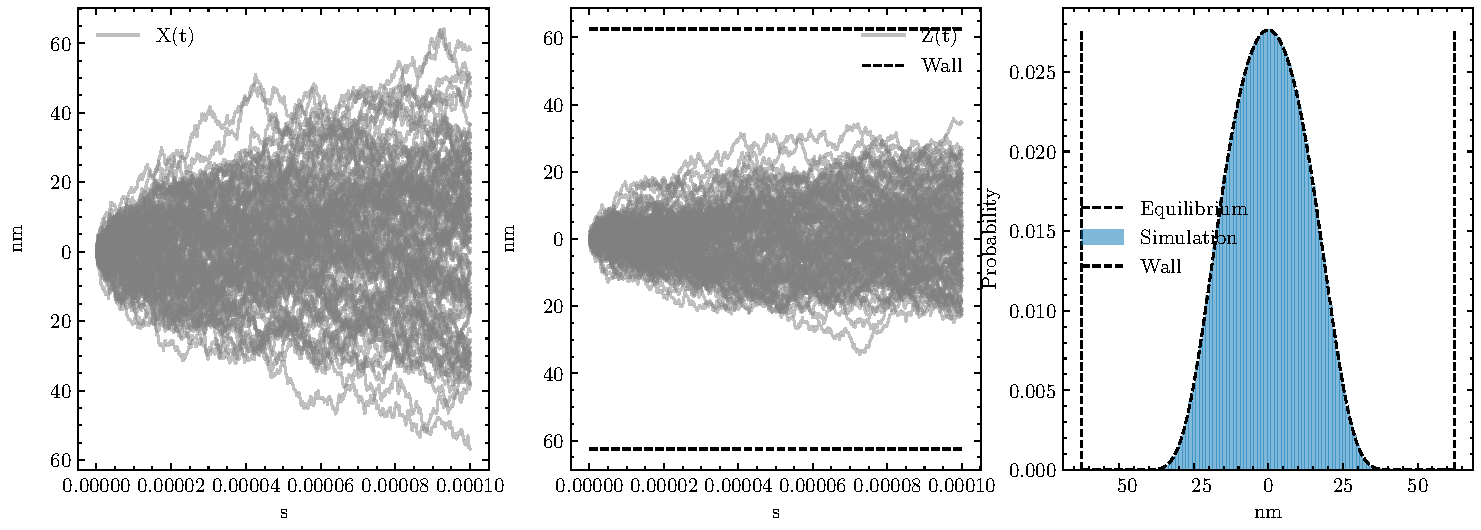
\includegraphics[width=\linewidth]{Figures/simulations/realization_and_boltzmann.pdf}
    \caption{Confined Brownian Particle realization of $z$ diffusion in electrostatic potential. $a = \SI{50}{\nm}, \zeta_p = \SI{-30}{\milli \volt}, \sigma_w = \SI{-2}{\milli \coulomb / \meter^2}, L = \SI{225}{\nm}, \lambda_D = \SI{10}{\nm}, T = \SI{300}{\kelvin}, \eta = \SI{1}{\milli \pascal \second}$. Left. Particle trajectory vs time for 100 realizations. Right. Histogram of steps vs. Boltzmann distribution.}
    \label{fig:brown_realization}
\end{figure}

\section{Mean-Squared Displacement in Confinement}

For a given experiment, one aims to measure something from knowing the trajectory of the particle. The simplest is an estimate of the size of the particle. One can do this using the transverse and axial trajectories obtained from the Langevin equation as a method to test the variance of the estimator given a known ground truth. In the case of an electrostatic potential, we can directly how measurements which do not account for screening effects change the measurement. 

\begin{figure}[h]
    \centering
    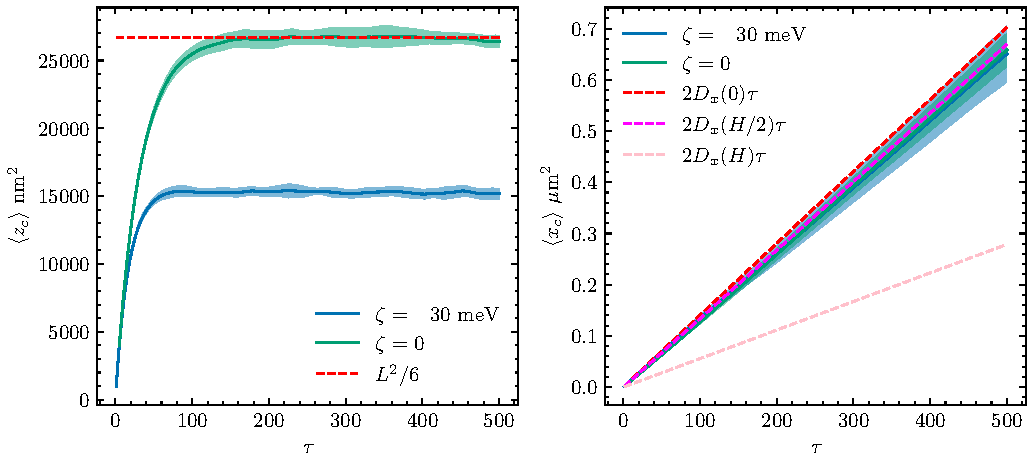
\includegraphics[width=\linewidth]{Python/Figures/xz_msd_comparison.pdf}
    \caption{Comparison between MSd curves of two highly different confined diffusors. Exposure time $\tau = \SI{200}{\micro \second}$, $\lambda_D = \SI{10}{\nm}$. }
    \label{fig:xz_msd_comparison}
\end{figure}

The notation of a higher confinement with respect to the zeta-potential is intrinsically linked to the electrostatic potential that the particle feels as it explores the well. This relationship between the effective confinement length can be solved by solving the Green's function for the FP-equation in the presence of an electrostatic potential. However, this happens to be non-analytical in the case of the Poisson-Boltzmann potential approximated in the Debye-Huckle theory. However, using the developed simulation class, this relationship can be directly measured. The same settings were used while fixing the zeta-potential of the particle, and varying the ionic concentration of the solution, which is inversely proportional to the Debye-length,
\begin{equation}
    \lambda_D \propto \frac{1}{\sqrt{C}},
\end{equation}
where $C$ is the ionic concentration of a dilute electrolyte compound [CITE]. To model this, the simulation settings are chosen as such $a = \SI{50}{\nm}, L = \SI{500}{\nm}, T = \SI{300}{\kelvin}, \Delta t_i = \SI{0.2}{\micro \second}, \tau = \SI{200}{\micro \second}, \eta = \SI{1}{\milli \pascal \second}$ and the Debye length is varied. The zeta potential of the particle and glass are chosen to resemble glass and a polystyrene bead, fixed at $\sigma_w = \SI{-2}{\milli \coulomb / \meter^2}, \zeta = \SI{-30}{\milli \volt}$. The relationship between the effective confinement length and the ionic concentration is shown in Fig. \ref{fig:conf_debyelen}

\begin{figure}
    \centering
    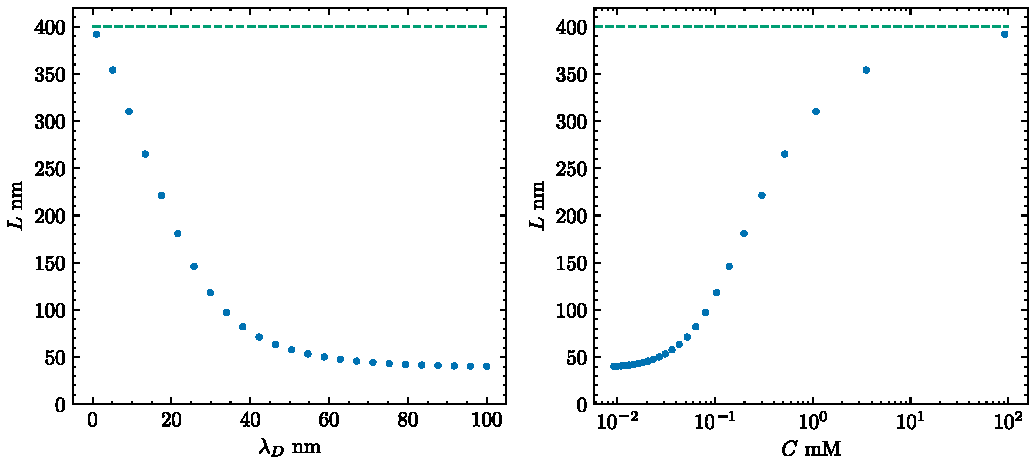
\includegraphics[width=\linewidth]{Python/Figures/conf_debyelength.pdf}
    \caption{Effective Confinement length plotted against the solution's Debye length. $a = \SI{50}{\nm}, L = \SI{500}{\nm}, T = \SI{300}{\kelvin}, \Delta t_i = \SI{0.2}{\micro \second}, \tau = \SI{200}{\micro \second}, \eta = \SI{1}{\milli \pascal \second}$ and the Debye length is varied. The zeta potential of the particle and glass are chosen to resemble glass and a polystyrene bead, fixed at $\sigma_w = \SI{-2}{\milli \coulomb / \meter^2}, \zeta = \SI{-30}{\milli \volt}$. }
    \label{fig:conf_debyelen}
\end{figure}

\begin{figure}
    \centering
    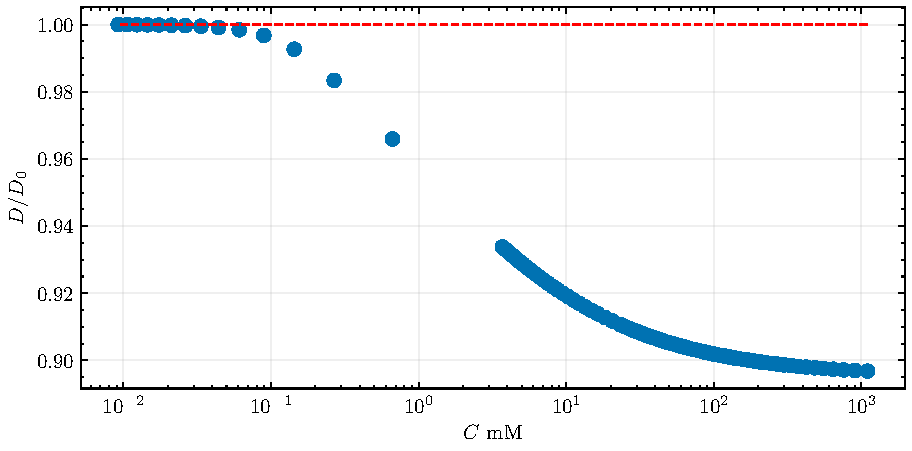
\includegraphics[width=\linewidth]{Python/Figures/diff_debye.pdf}
    \caption{Effective diffusion plotted against the solution's Debye length. $a = \SI{50}{\nm}, L = \SI{500}{\nm}, T = \SI{300}{\kelvin}, \Delta t_i = \SI{0.2}{\micro \second}, \tau = \SI{200}{\micro \second}, \eta = \SI{1}{\milli \pascal \second}$ and the Debye length is varied. The zeta potential of the particle and glass are chosen to resemble glass and a polystyrene bead, fixed at $\sigma_w = \SI{-2}{\milli \coulomb / \meter^2}, \zeta = \SI{-30}{\milli \volt}$. }
    \label{fig:diff_debyelen}
\end{figure}

The relationship between the effective confinement length, as well as the relationship between relative diffusion and concentration of ions begs the question of if this can be used as a particle filter to distinguish classes of particles. Here we investigate that question regarding the amount of confinement length compared to the zeta-potential of a particle at various Debye-lengths. This relationship is described in Fig. \ref{fig:conf_zeta_debye}.
\begin{figure}
    \centering
    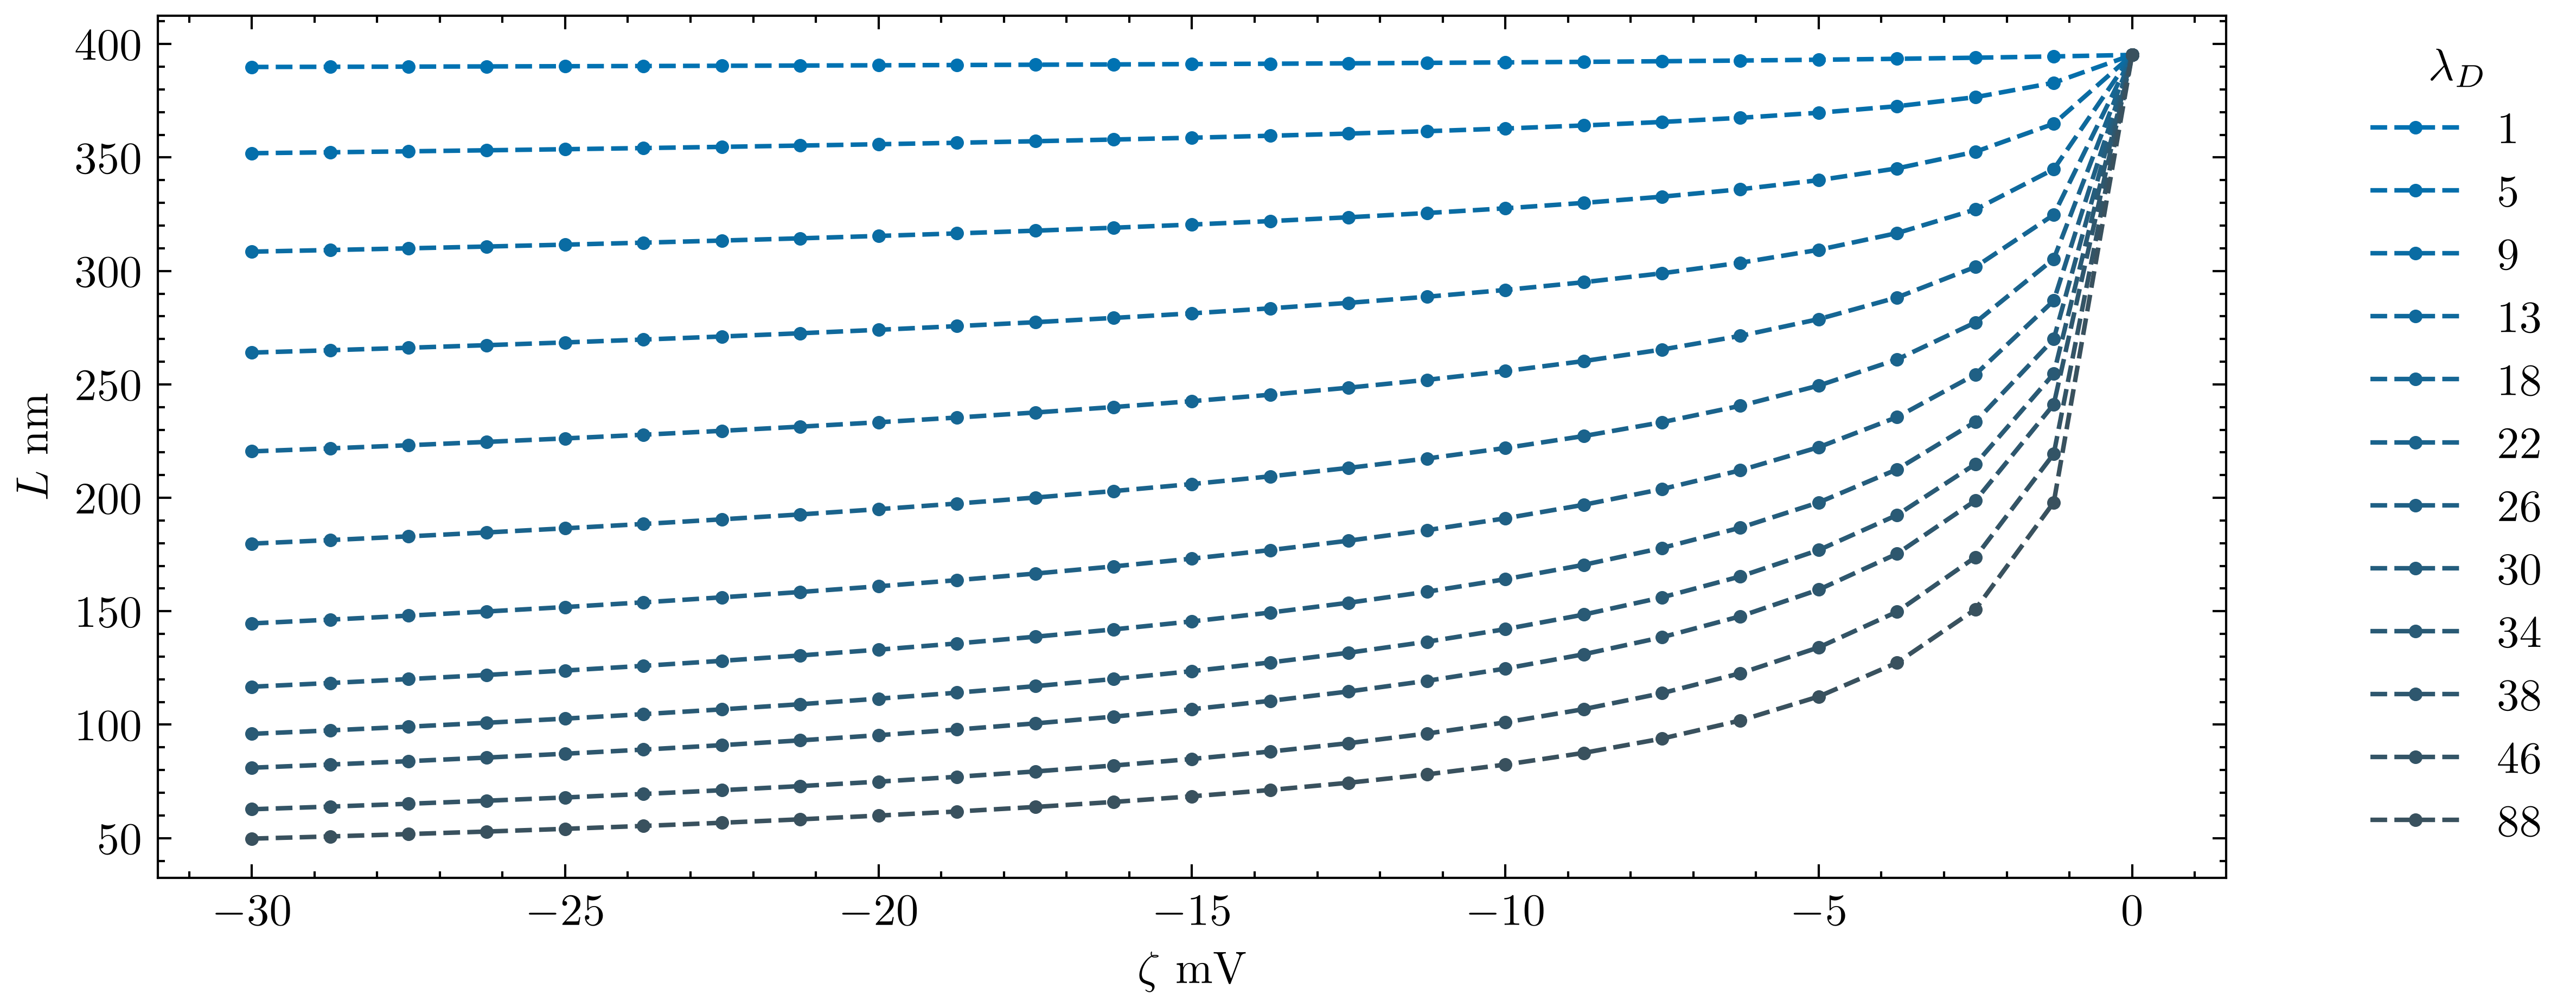
\includegraphics[width=\linewidth]{Python/Figures/conf_zeta_debye.png}
    \caption{Effective confinement plotted against the particle's zeta-potential. $a = \SI{50}{\nm}, L = \SI{500}{\nm}, T = \SI{300}{\kelvin}, \Delta t_i = \SI{0.2}{\micro \second}, \tau = \SI{200}{\micro \second}, \eta = \SI{1}{\milli \pascal \second}$ and the Debye length is varied. The surface charge of the wall are chosen to resemble glass, fixed at $\sigma_w = \SI{-2}{\milli \coulomb / \meter^2}$.}
    \label{fig:conf_zeta_debye}
\end{figure}

\section{Surface Charge estimation}

The particle's exploration demonstrated a clear dependence on a drift due to the electrostatics. This drift is a useful estimator of the particle-wall charge relationship. Using the aforementioned amplitude maximum-likelihood estimator, drift estimator can be extracted into meaningful, physical information. The Langevin simulation was ran for $\SI{20}{\ms}$ with time-step of $\SI{0.2}{\micro\second}$. The distribution of the MLE is shown in Fig \ref{fig:B_estimation}.

\begin{figure}[hb]
    \centering
    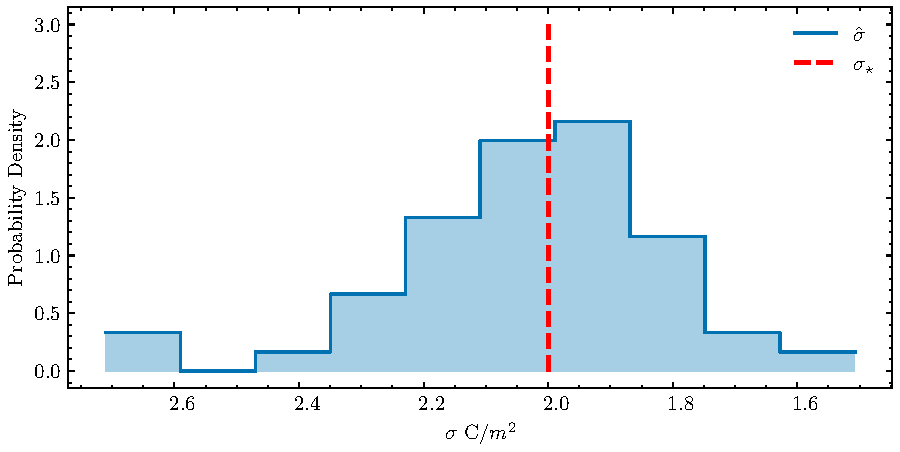
\includegraphics[width=0.75\linewidth]{Python/Figures/B_estimation_hist.pdf}
    \caption{Distribution of $\hat{B}$ Re-parameterized for the surface charge. $\hat{\sigma} = 1/(A\cdot C)^2 \hat{B}$ where $A,C$ are properly defined in \ref{eqn:electrostatic_forces}. In this histogram there are 50 simulations with seeds set to $S_{\text{eed}} = i* 10 + 1$ for $i \in \{0, 49\}$ using the \textit{numpy} seed parameter. $a = \SI{50}{\nm}, L = \SI{500}{\nm}, T = \SI{300}{\kelvin}, \Delta t_i = \SI{0.2}{\micro \second}, \tau = \SI{200}{\micro \second}, \eta = \SI{1}{\milli \pascal \second}, \lambda_D = \SI{10}{\nm}$ The surface charge is fixed at $\sigma_w = \SI{-2}{\milli \coulomb / \meter^2}$.}
    \label{fig:B_estimation}
\end{figure}

\section{Conclusion}

In conclusion, we have shown that confined simulations can be readily simulated with physical parameters as per literature. The simulations have shown that there are regions of instability in the Debye-surface charge regime where the confined diffusivity of the particles is maximally observed. For the case of polystyrene beads, this appears to be around $\lambda_D \approx \SI{80}{\nm}$. 

With regards of surface charge estimation, we have introduced a new MLE for the amplitude based on maximum likelihood estimation. The distribution has a mean centered around the ground truth with a standard deviation of $1/4 \cdot \sigma_\star$. 

\chapter{iSCAT z-estimation Simulations}
\label{chap:ZEstimation}

This section presents a computational method for determining the axial ($z$-axis) position of a nanoparticle from iSCAT imaging data. The proposed approach is based on principles of light-scattering in the Rayleigh approximation, which govern the inference pattern as the nanoparticle moves along the optical axis. 

In order to evaluate the accuracy and performance of the proposed method, Mie-theory simulations are used for for determining the an ideal nanoparticle's $z$-axis position. The precision and limitations are discussed in the context of recovering three-dimensional particle trajectories.

The raw images are acquired from a CMOS camera according the optical schematic illustrated in Figures \ref{fig:schematic} and \ref{fig:re_schematic}. Each image consists of a two-dimensional interference recorded at a specific focal position $z_\mathrm{focus}$, defined as the distance between the objective's focal distance and the objects in the field of view.

\section{Method Overview}

The method described in this section is based on computational image processing on images acquired using a CMOS camera. The camera has an array of $2048 \times 2048$ pixels. To acquire images at higher frame rates, only a portion of the CMOS array is used. This is set during the experimental details. Typical sizes used are $600 \times 450$ at $\SI{400}{\fps}$ however, other fields of view can be used for specific experimental purposes. The highest frame-rate possible with this camera is $\SI{1000}{\fps}$ at a FOV of $200 \times 250$.

The object sample is imaged through an oil-immersion objective lens. The optical system provides a magnification of $60 \times$, with a tube lens of magnification $2\times$. The remaining is an digital zoom with a final resolution of $\SI{55}{\nm}$ per pixel. The final magnification is then the ratio of the CMOS array length divided by the pixel size.

The image-processing workflow used to determine three-dimensional trajectory is shown in \ref{fig:method_outline}. The diagram summarized the sequence of image processing steps to extract each coordinate position.

\begin{figure}[h!]
    \centering
    \begin{minipage}{0.6\textwidth}
        \centering
        \begin{enumerate}
            \item Raw image captured on camera.
            \item Background subtraction to convert to iSCAT image.
            \item iSCAT $(x,y)$ Tracking
            \item Radial Integral to obtain scattering data.
            \item Nuisance parameter estimation to ensure physical stability.
            \item Particle axial position Linking with 2D chain-link algorithm.
            \item Axial position Extraction
            \item Three-dimensional trajectory is recovered.
        \end{enumerate}
    \end{minipage}
    \caption{Background subtraction outline. }
    \label{fig:method_outline}
\end{figure}


\section{Raw image background subtraction}

To obtain high-contrast interference signal from raw camera data, a post-processing background subtraction routine is introduced. This background subtraction measured a temporally averaged background using a window-filter and Fourier filtering. An example of this process is shown in Fig.\ref{fig:raw2iscat}.

\begin{figure}[h]
    \centering
    \begin{subfigure}[b]{0.8\textwidth}
        \centering
        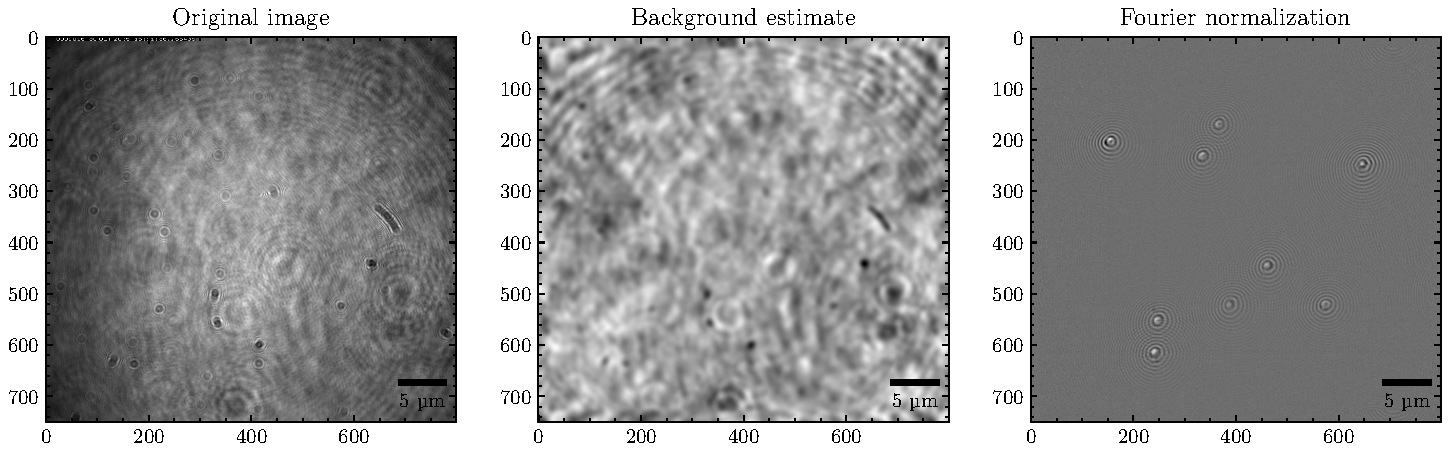
\includegraphics[width=\textwidth]{Python/Figures/NormalizationPipeline.pdf}
    \end{subfigure}
    
    \vspace{1em} % Adjust the vertical space between figures
    % Second (bottom) subfigure
    \begin{subfigure}[b]{0.5\textwidth}
        \centering
        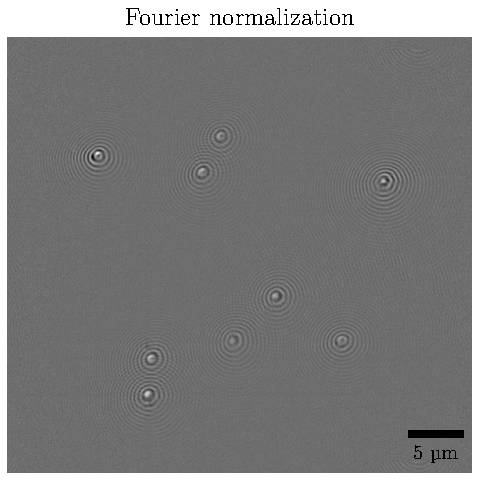
\includegraphics[width=\textwidth]{Python/Figures/NormalizationPipelineThird.pdf}
    \end{subfigure}

    \caption{Raw image captured on camera to background subtracted iSCAT image. Single particles are tracked and extracted for further analysis.}
    
    \label{fig:raw2iscat}
\end{figure}

The full algorithm is presented in Alg. \ref{alg:raw2iscat}. The overview of the algorithm is to subtract the background noise in order to minimize Poisson, and electronic noise. 

To reduce the contribution of the static background, the mean background is subtracted from each frame. Since the background illumination originates from the gaussian illumination beam, which has a constant mean intensity over the acquisition period, this stationary background removes the background offset while preserving dynamic iSCAT signal. This just requires a good estimation of the background in order not to remove any iSCAT signal. The remaining shot noise, which follows Poisson statistics is reduced by temporal averaging during background estimation. 

In order to suppress electronic noise from data-transfer, a row-wise averaging scheme is applied. Row-wise means are taken and normalized with respect to their row as the data-transfer from CMOS to computer is by horizontal lines. Thus, to ensure all lines are equally weighted, they are normalized with respect to their entire row. This is implemented as per prior iSCAT normalization methods by the Sandoghar laboratory \red{Vahid's github should be here.}

The set of images, which consist of matrices of pixel-values of shape $F \times H \times W$, or $F$ number of frames, $W$ pixels wide, $H$ pixels tall. 

Before processing begins, the parameters of the Fourier-band-pass filter are determined from the image dimensions. The filter consists of an annular, donut mask of inner radius equal to 1\% if the larger image dimension and outer radius equal to  25\% of the larger image dimension, corresponding to $r_i = \max(H,W)/100, r_o = \max(H,W)/4$. 

To minimize edge artifacts, a binary mask is applied to each frame. Pixels within 20 pixels of the boundary are assigned a value of 0 using a mask filter. On the interior pixels, the mask is set to $1$, while on the pixels less than 20 pixels away from the edge are set to 0. This mask is used during normalization to prevent edge effects from biasing the inner statistics.

For each frame in the stack, the image is first normalized using a row-wise normalization function. The function, titled \textsc{AmpNorm} in Alg. \ref{alg:raw2iscat}, first obtains the masked-image. The global normalized mean is stored. For each row, the mean is taken and the row of the global-mean is adjusted by the row-wise mean. The final image is the global mean divided by the row-mean for each row. 

Once normalized, the background of the image is calculated by taking the forward and backward $\Delta L$ frames spaced by a spacer of $\Delta f$ frames and taking the $\textsc{AmpNorm}$ of these frames. 

The iSCAT image then consists of a background subtraction between the normalized image and the background. Finally, once background subtracted, the image is Fourier-filtered using the pre-allocated band-pass filter. This process is demonstrated in Fig. \ref{fig:raw2iscat}

\section{iSCAT $(x, y)$ Tracking}

To determine the transverse positions of any particles detected in the iSCAT method, the radial variance transform algorithm is used \cite{kashkanovaPrecisionSingleparticleLocalization2021}. The original algorithm is briefly outlined below for completeness. The full code is written by the Sandoghdar group and can be found in Ref \cite{kashkanovaPrecisionSingleparticleLocalization2021}. A demonstration of this method is presented in the Fig. \ref{fig:transLoc}.

\begin{figure}[h]
    \centering
    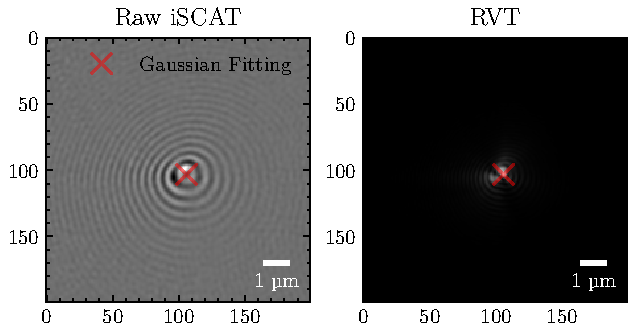
\includegraphics[width=\textwidth]{Python/Figures/Raw2RVT.pdf}
    \caption{Raw image to RVT. Gaussian fitting of the RVT is shown on both plots.}
    \label{fig:transLoc}
\end{figure}

The transverse localization algorithm, referenced as \textsc{TransverseLocalization} in \ref{alg:2d_track} consists of transformations onto the iSCAT image from the previous section. 

The input image stack is first loaded and assumed to consist of radially symmetric interference fringes. The image is first transformed using the Radial Variance Transform \cite{kashkanovaPrecisionSingleparticleLocalization2021}. This function converts a radial-fringe pattern into a point-like delta function when a radial symmetry is acted upon it. 

Before proceeding, a frame-independent parameter for threshold SNR amplitude, number of pixels, and ROI cropping parameters are inputted. for a particle to be detected, the SNR of the RVT should be roughly 90\% of the max iSCAT amplitude. An estimate of particle number is assumed, which acts as a prior for top $n$ detections. Lastly, ROI for sub-pixel estimation is chosen. 

For each frame, the iSCAT image is dilated. Particle positions that are considered maxima if the dilated image is equal to the RVT and the RVT is above the threshold for detection. 

Once candidates are chosen, a NL-LS gaussian fitting to the RVT is performed to acquire higher-accuracy localization. To improve this to sub-pixel, a crop is done around each RVT gaussian fitted point and a radial-symmetry algorithm is performed as per \cite{parthasarathyRapidAccurateParticle2012}.

\begin{figure}
    \centering
    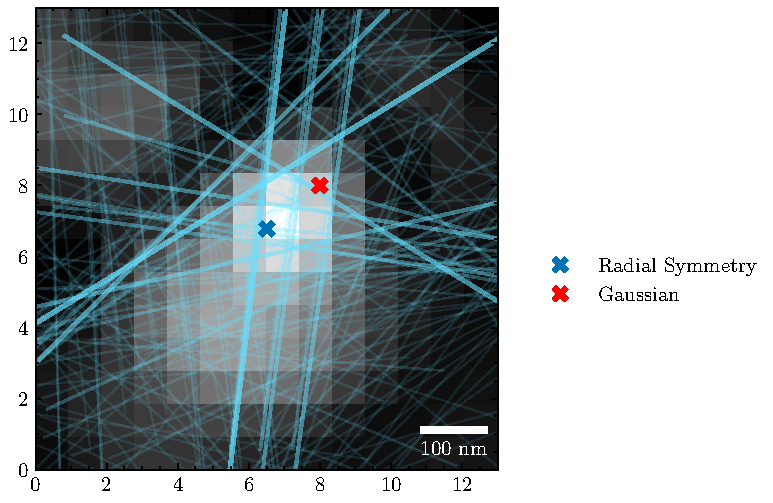
\includegraphics[width=0.8\textwidth]{Python/Figures/RadialSymExample.pdf}
    \caption{Demonstration of the Radial Symmetry method applied onto RVT of iSCAT data. Implemented from \cite{parthasarathyRapidAccurateParticle2012}. Figure adapted from \cite{parthasarathyRapidAccurateParticle2012}.  }
    \label{fig:RadialSym}
\end{figure}

To ensure accurate linking, an implementation of the \textsc{Munkres} algorithm is used \red{REF}. Briefly, a cost-matrix of distances is constructed and minimized in time to ensure that optimal displacements are chosen. This algorithm has limitations in cases where particles overlap. Ideally, experimental measure are taken to minimize this occurring. One such measure is to lower the concentration of particle in the recorded images. 



\section{Angular Integral}

Image data will have background misalignment due to iSCAT hardware setup. To optimize for fitting speed and misalignment property, radial scattering profile are assumed as in the Rayleigh regime model is symmetric. The radial integration method is described in Alg \ref{alg:rad_int}.

The discrete angular integral consists of summing angular terms on a radial grid. Mathematically, the output array obtained is described by the relation
\begin{equation}
    g_t(\rho) \tilde{-} \frac{1}{\Delta \theta}\int_{\theta_0}^{\theta_0 + \Delta \theta} I_t(\rho, \theta) d\theta,
\end{equation}
where $\theta_0$ is a constant, $\Delta \theta$ is the width of integration, $I_t(\rho, \theta)$ is the iSCAT image. 

First, the cartesian image is Re-parameterized into polar coordinates using a change of basis transformation on the index grid of the image. Then, for each ring of indices, the image coordinates are summed up on this ring. The final array is an angular average that is indexed at radius $r$ for some upper radial bound. This process is illustrated in Fig. \ref{fig:AngularInt}.

\begin{figure}[h!]
    \centering
    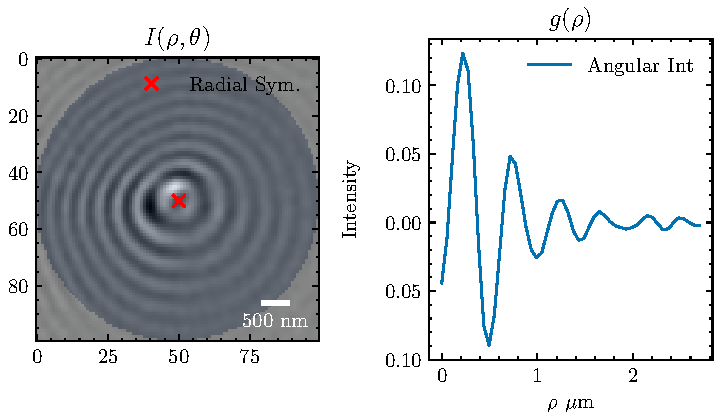
\includegraphics[width=\textwidth]{Python/Figures/AngularInt.pdf}
    \caption{Angular Integral demonstration.}
    \label{fig:AngularInt}
\end{figure}

\section{Nuisance parameter Estimation}

In order to speed up computation and produce a more statistically relevant result, the method aims to fix the model parameters which should theoretically stay constant. These, for example, are the particle mass signal and optical aberration coefficients. These parameters, known as nuisance parameters, should be fixed before fitting to the more sensitive parameter of interest, the relative $z$ position. 

To obtain accurate estimation of the $z$ position relative to nearby frames, nuisance estimation is done to focus on $z$ fitting. To do this, L-BFGS-B Fitting is performed. alongside amplitude fitting. The theory of nuisance parameter estimation is described in \cite{wasserman2010statistics}.

The nuisance parameter method works on the premise of a model function. The iPSF model described in \ref{chap:iscatprinciples} is used as a weight function to compare to the data. First, bounds are placed for physical values of each parameter.

Here, it is important to note that the amplitude of the signal is proportional to the mass. The spatial decay of the aberration is modeled as a decaying exponential.

For each candidate decay parameter, the weighted correlation function is calculated. Let $g$ be the radial profile, and $G$ the theoretical iPSF model. The inner product of these two arrays, weighted in some integral of radiuses, is defined by $\langle G, g \rangle_w$. The correlation function is then written as
\begin{equation}
    \rho(z, \gamma) = \frac{\langle G, g \rangle_w}{\sqrt{\langle G, G \rangle _w + \langle g, g \rangle_w + \varepsilon}},
\end{equation} 
where $\varepsilon$ is a small number to prevent division by 0. 

The best-fit amplitude function here is analytical, given by the expression
\begin{equation}
    \hat{E_0} = \frac{\langle G, g \rangle_w}{\langle G, G \rangle_w}.
\end{equation}

The loss-function, $\mathcal{L}$, given the correlation, is given by the subtraction of $\rho^2$,
\begin{equation}
    \mathcal{L} = 1-\rho^2(z, \gamma).
\end{equation}

Once a fitted $\gamma_0, \hat{E_0}$ are chosen, the optimal $z$ for each frame is given by a non-linear bounded least squares which are acquired using the L-BFGS-B method with a Huber Loss ($\delta = 1/2$). 

When computed for each frame in the stack, one has $F$ optimally chosen $\gamma_0, E_0$. To obtain the optimal parameter, a fit to distributions, inferred by \cite{dewitPreciseCharacterizationNanometerscale2023}, is used. These fits include a Gamma distribution for $E_0$ and a LogNorm distribution for $\gamma$. Together, these form nuisance estimation for $E_0, \gamma_0$.

\section{2D Chain-link}

Given an estimation of the nuisance parameters, a grid-search of the optimal $z$ is simple. The physically best $z$ position is a mean-squared error loss minima of the model subtracted with the data. However, due to the periodic nature of the data, there are up to 3 candidates for the optimal $z$ position based on $\lambda/4$ having a high degree of similarity. Thus, to resolve this, a z-linking method was implemented to find the most likely trace based on diffusion probabilities.

To link consequent positions in space, a dynamic programming algorithm is used. The algorithm is known as the Viterbi method and is described in Alg. \ref{alg:best_chain_2d}.

First, all minima for every frame must be collected. These are the candidate positions that trajectories are constructed from. The losses of these positions are also stored to ensure no spurious candidates are chosen. 

For each position, the forward pass compares all chains moving in time. The loss is accumulated by a weighted Euclidean transition cost,
\begin{equation}
    d_i(i,j) = \sqrt{w_x^2(x_{t-1}^(i) - x_{t}^(j))^2 + w_y^2(y_{t-1}^(i) - y_{t}^(j))^2},
\end{equation}
where $x$ denote $z$ motion, and $y$ denotes the loss difference. This matrix compares all weighted transitions. The optimal transition $\pi_t(j)$ is then chosen to minimize this transition, and any prior transitions. 

For each following forward pass, the cost is accumulated with a memory of 2 frames. The memory is chosen to ensure that an incorrect transition in a given frame is not penalized later on. 

Thus linking method is thus a search algorithm for the shortest math based on the weighted Euclidean method. A short toy-model is shown in Fig. \ref{fig:toyViterbi} to visualize the procedure.

\begin{figure}[H]
    \centering
    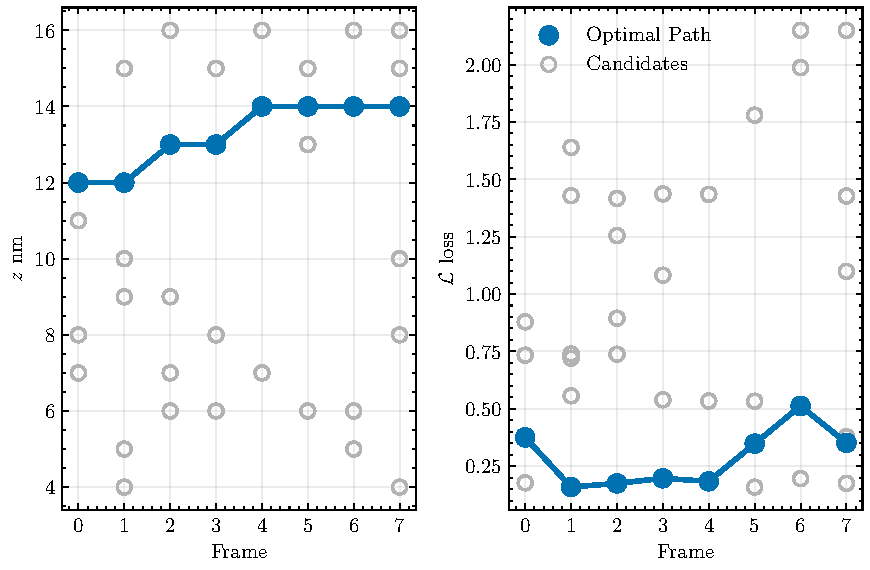
\includegraphics[width=0.8\textwidth]{Python/Figures/viterbi_toy.pdf}
    \caption{Viterbi Search algorithm toy example. Optimal path is chosen based on $z$ similarity and lowest loss.}
    \label{fig:toyViterbi}
\end{figure}

% \begin{algorithm}[H]
% \caption{Dynamic Programming for Best 2D Chain of Points}
% \label{alg:best_chain_2d}
% \begin{algorithmic}[1]
% \Require 
%     $\text{min\_idx} = \{ \text{min\_idx}[t] \}_{t=0}^{F-1}$, list of candidate positions per frame\\
%     $\text{min\_vals} = \{ \text{min\_vals}[t] \}_{t=0}^{F-1}$, list of candidate values per frame\\
%     $w = (w_x, w_y)$, weighting for distance computation (default $(1,1)$)\\
%     $\text{max\_step}$, optional maximum allowed step distance
% \Ensure
%     $\text{idx\_chain}, \text{x\_chain}, \text{y\_chain}$, the indices, positions, and values of the optimal path

% \State Initialize $F \gets |\text{min\_idx}|$
% \State Initialize $cost[i] \gets 0$ for all $i$ in frame $0$
% \State Initialize $prev \gets []$ \Comment{to store predecessor indices}

% \For{$t = 1$ to $F-1$}
%     \State $A_x \gets \text{min\_idx}[t-1]$, $B_x \gets \text{min\_idx}[t]$
%     \State $A_y \gets \text{min\_vals}[t-1]$, $B_y \gets \text{min\_vals}[t]$
%     \State Compute pairwise differences:
%         \[
%         \Delta_x[i,j] = |A_x[i] - B_x[j]|, \quad 
%         \Delta_y[i,j] = |A_y[i] - B_y[j]|
%         \]
%     \State Compute weighted Euclidean distances:
%         \[
%         D[i,j] = \sqrt{ (w_x \Delta_x[i,j])^2 + (w_y \Delta_y[i,j])^2 }
%         \]
%     \If{max\_step is not None}
%         \State Set $D[i,j] \gets \infty$ if $D[i,j] > \text{max\_step}$
%         \If{no finite $D[i,j]$ exists}
%             \State \Return empty path
%         \EndIf
%     \EndIf

%     \State Compute cumulative path cost matrix:
%         \[
%         M[i,j] = cost[i] + D[i,j]
%         \]
%     \State For each node $j$ in frame $t$, find predecessor $p[j]$ minimizing $M[:,j]$:
%         \[
%         p[j] = \arg\min_i M[i,j], \quad
%         new\_cost[j] = M[p[j], j]
%         \]
%     \State Update $cost \gets new\_cost$
%     \State Append $p$ to $prev$
% \EndFor

% \State Initialize $j \gets \arg\min_i cost[i]$  \Comment{index of minimal total cost in last frame}
% \State Initialize $\text{idx\_chain} \gets [0]^{F}$, set $\text{idx\_chain}[F-1] \gets j$
% \For{$t = F-2$ down to $0$}
%     \State $\text{idx\_chain}[t] \gets prev[t][\text{idx\_chain}[t+1]]$
% \EndFor

% \State Compute chains:
% \[
% \text{x\_chain}[t] = \text{min\_idx}[t][\text{idx\_chain}[t]], \quad
% \text{y\_chain}[t] = \text{min\_vals}[t][\text{idx\_chain}[t]]
% \]

% \State \Return $\text{idx\_chain}, \text{x\_chain}, \text{y\_chain}$
% \end{algorithmic}
% \end{algorithm}

\section{Simulated iPSF localization}

To validate the proposed method, one performs simulated axial-estimation. Simulated iSCAT point spread functions were generated using the \textsc{PiSCAT} library for $\lambda=\SI{405}{\nm}$. The iPSF was generated for the focal range $z_{f} \in [-1000, 0]$. The assumed particle is spherical with radius $a = \SI{50}{\nm}$. The iPSF is shown in Fig. \ref{fig:ipsf_sim}

\begin{figure}
    \centering
    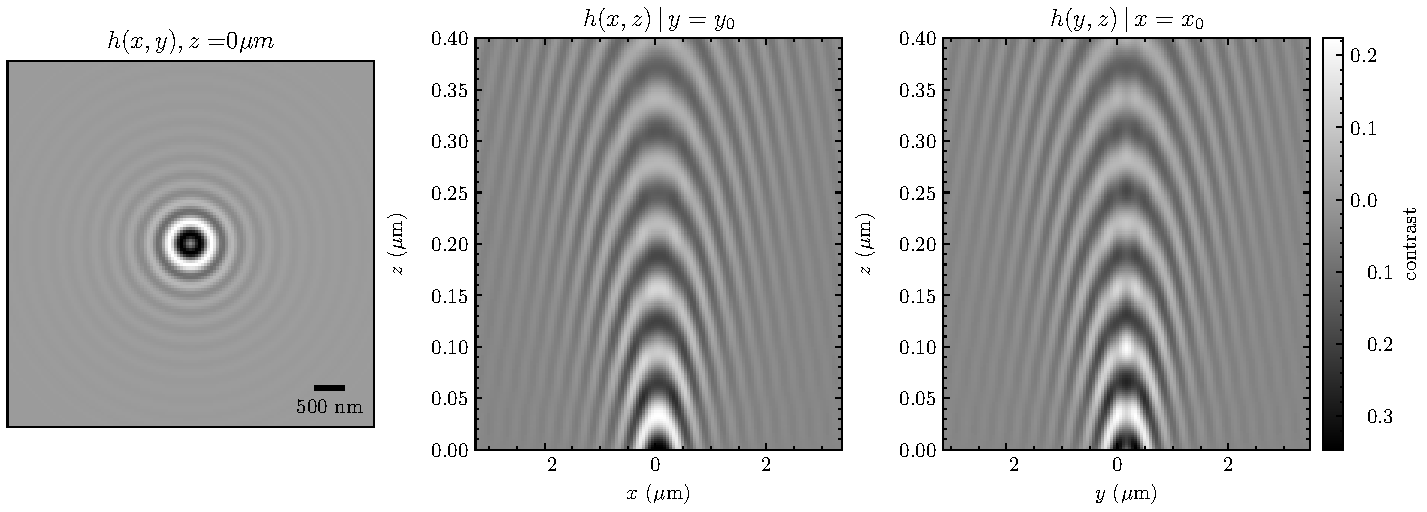
\includegraphics[width=\linewidth]{Python/Figures/sim_ipsf.pdf}
    \caption{Simulated iPSF. Left. Projection of in-focus plane. Middle. $x,z$ projection. Right. $y,z$ projection. Focal scan is over $\SI{400}{\nm}$. pixel size is $\SI{55}{\nm}/\text{pixel}$. $\lambda = \SI{405}{\nm}$. Assumed particle radius $a = \SI{50}{\nm}$.}
    \label{fig:ipsf_sim}
\end{figure}

As mentioned, the localization pipeline utilizes a weighting scheme to account for objective aberration and misalignments to non-modeled regions of the data, such as the central fringe. This is accounted for by using a binary weighting array, $\mathbf{w}$. In the case of these idealized simulations, we will show the effect of changing the weighting scheme as we proceed. This demonstrates a loss of absolute precision, however, maintains the relative precision, which is that of interest in measurements of axial trajectory. 

\section{3-parameter Estimation}

As a reminder, the model for the iPSF is a multivariate function $\text{iPSF}:(z, E_0, \gamma) \rightarrow \R^2$. It has been shown that the statistical model of $\text{iPSF}$ takes;
\begin{equation}
    \begin{aligned}
        \hat{E_0} &\sim \text{Gamma}(\mu_{E_0}, \sigma_{E_0}) \\
        \hat{\gamma} &\sim \text{logNorm}(\mu_{\gamma}, \sigma_{\gamma}) \\
    \end{aligned}
\end{equation}

The so-called 3-parameter estimation is a sampling of nuisance parameters in the model. The nuisance parameters here are $\hat{E_0}, \hat \gamma$, where $\hat{E_0}$ is an amplitude factor, and $\gamma$ is an exponential decay factor used to account for spatial decay in signal. The amplitude factor can be analytically solved for using a grid-search sweep along $z$. The $\gamma$ factor is fitted to using the L-BFGS-B minimization algorithm. This nuisance parameter fit is shown in the histograms of these two parameters shown in Fig. \ref{fig:nuisance_fit}.

\begin{figure}
    \centering
    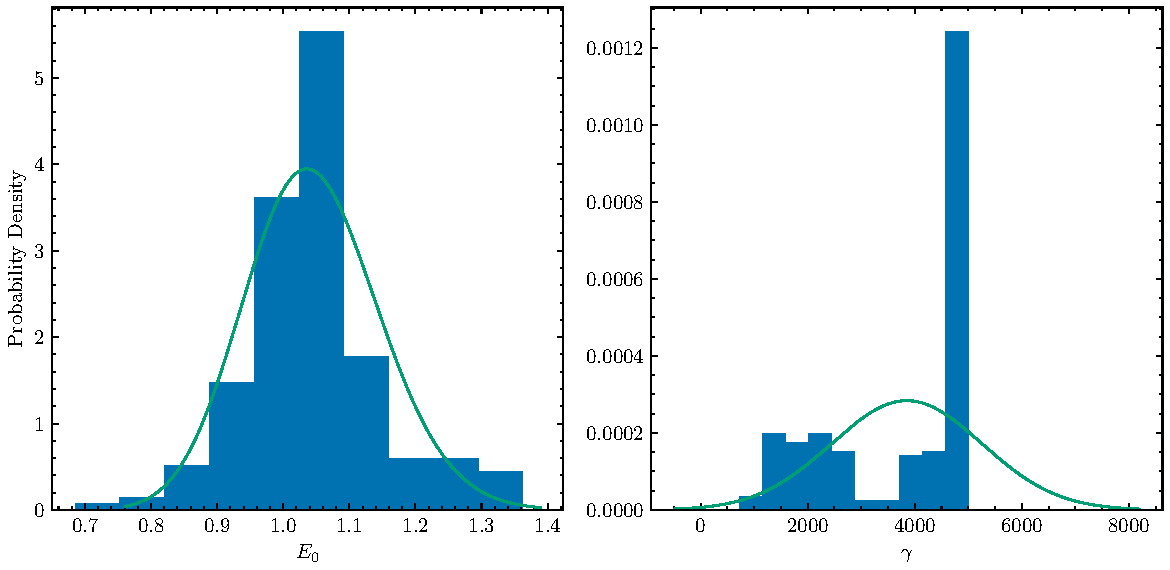
\includegraphics[width=\linewidth]{Python/Figures/nuisance_param.pdf}
    \caption{Nuisance Parameter estimation for iPSF fits. Left. Amplitude factor. right. exponential decay factor. The exponential decay is not of utmost importance as it often is very small. it is kept for stability purposes.}
    \label{fig:nuisance_fit}
\end{figure}

\subsection{Grid-Search Estimation}

Once the nuisance parameters are chosen, a grid-search with a dynamic linking is performed. Each frame is assumed to have a maximal diffusion time. This is in place to optimize for noise and have coherent, physical traces without outliers. The grid search takes the difference between the data and a scan over the model with the nuisance parameters in place. The best loss is chosen. In the case of linking, the minimal loss over the path is chosen. The full algorithm is discussed elsewhere. the residuals of this using no fitting are shown in Fig. \ref{fig:fit_residuals}.

\begin{figure}
    \centering
    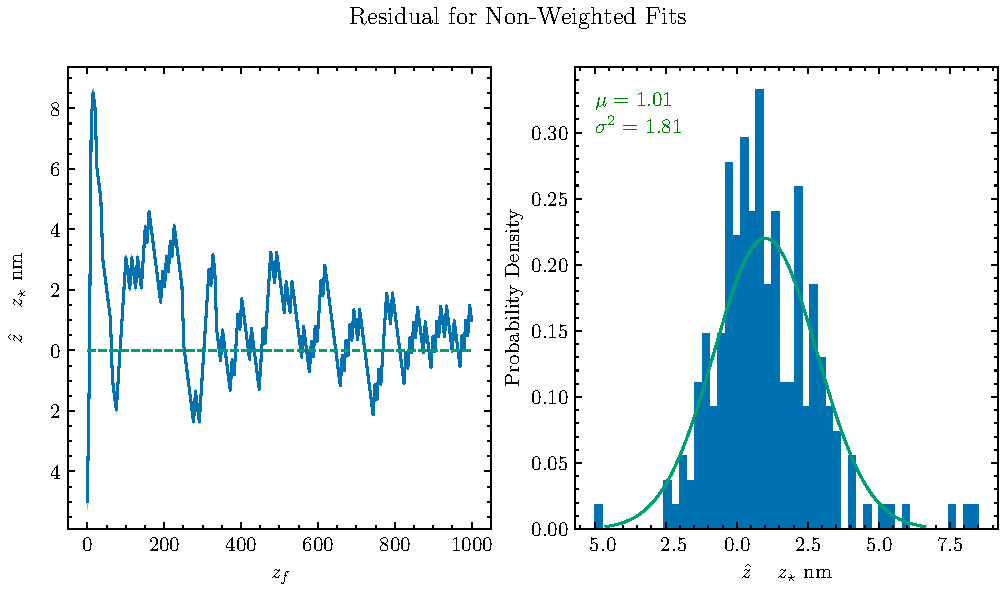
\includegraphics[width=\linewidth]{Python/Figures/simulation_fit_residual.pdf}
    \caption{Fit residuals using no weighting scheme. reporting an absolute bias of 1 nm with variance of 2 nanometers.}
    \label{fig:fit_residuals}
\end{figure}

\section{Conclusions}

In conclusion, the pseudocode for the method was outlined explicitly. The methodology was tested on simulation data with a high degree of accuracy. The method shows an accuracy of $\pm \SI{1}{\nm}$ with a forward bias of $\SI{1}{\nm}$.





    \chapter{Widefield backscattering iscat for SPT in 3d confinement tracking and analysis}
    \section{Summary}

This work is ongoing and is in preparation for publication.

The goal of this work is to investigate and measure the size-diffusivity relationship of single-molcules in a confined environment. The goal of this project was to better understand the biases, variance, and details of size measurements performed by convex-lens induced confinement (CLiC). 

This study overviews a the dynamics on a model particle, which was chosen as plastic beads. The ionic concentration, as discussed in Chp. [5], is very important in focusing particles into an effective confinement length. This paper tends to evalute this model experimentally, as the Langevin model, although complete, is not-trivial in fuzzy/applied systems. To show this, the method is applied to 3 species of lipid-nanoparticle sample - liposomal, spherical, and bleb-like topologies.

During experimental trails, it has been found that these samples tend to stick to negatively charged surfaces, such as negatively charged cover glass, due to Van der Walls forces and electrostatic interactions. Over the last decade, passivation methods were used to alleviate this sticking. This paper aims to measure these interactions to determine the biases on size characterization associated with measuring molecule size in systems with these passivation methods. 


\section{Methods}

The following section outlines the tools used to collect data for this thesis. 

\subsection{Aparatus schematic}

The schematic of the system is Here we re-draw Fig \ref{fig:schematic} to remind the reader of the system. The optical system used for imaging is an iSCAT microscope. 

The optical system consisted of a $\SI{405}{\nm}$ excitation laser. The output of the laser was $\SI{240}{\milli \watt}$ pre-spatial filter, with an output of $\SI{120}{\milli \watt}$ post-spatial filter. The objective used was the $100 \times$ oil imaging objective (Nikon, Apochromat TIRF $100 \times$ oil immersion objective N.A. 1.49, W.D. $\SI{0.12}{\mm}$, F.O.V $\SI{22}{\mm}$). The camera used was the (\textcolor{red}{PRODUCT ID}) CMOS camera. Operating software was custom written by (\textcolor{red}{Author}) in LabView. 

\begin{figure}[t]
	\centering
    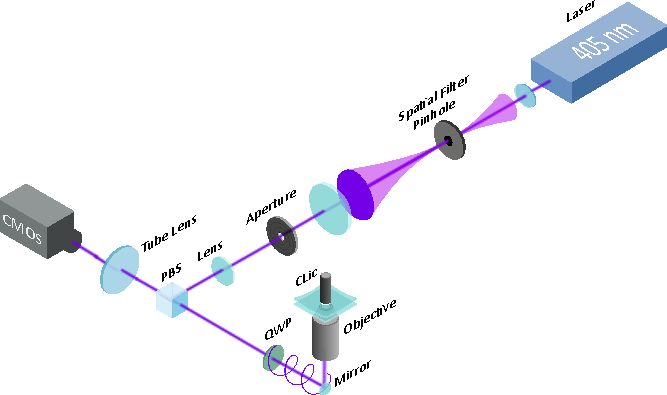
\includegraphics[width=\linewidth]{Figures/schematic}
    \caption{ iSCAT Schematic. A 405 nm laser is sent through a spatial filter, passes through an aperture. The beam is sent through a focusing lens which is reflected off a polarizing beam splitter, polarized through a QWP focused on the back plane of the objective. The scattered light is then polarized again, passing through the polarizing beam splitter and is focused on the CMOS camera. The final image is collected via the CMOS and saved in binary format.}
	\label{fig:re_schematic}
\end{figure}


\subsection{Cover-Glass}

The flow-cell device consisted of two glass substrates (Ted Pella, product no.260372, $145 \pm \SI{15}{\micro \meter}$ thick, $25 \times \SI{25}{\mm}$ cover glass), separated by a 30 um thick double-sided adhesive spacer (Nitto Denko, product no. 5603). 

\subsection{Convex-lens induced confinement}

The CLiC system was used to achieve nanometer confinement while imaging. This method is described in detail in the seminal publication \cite{berardPrecisionPlatformConvex2013}. A convex pusher lens is used together with a piezo linear actuator to displace the top coverslip of the flow-cell in a parabolic displacement. The pieze actuator is manually controlled during imaging and set to a specific, controlled height. The height is determined using the inference fringes of Newton's rings. The full method outline is visualized in Fig. \ref{fig:c7_fig1}


\begin{figure}
    \centering
    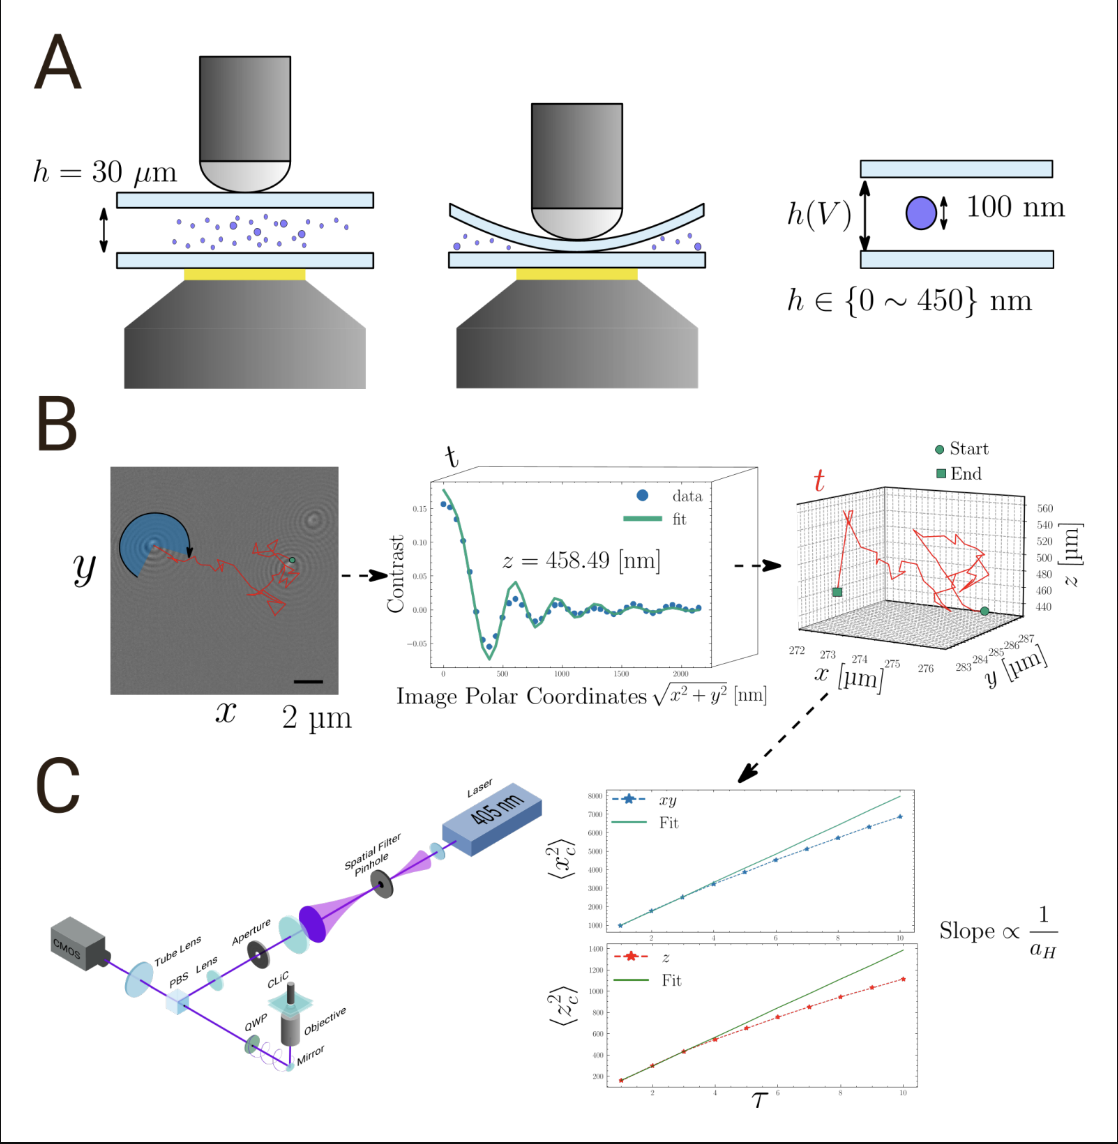
\includegraphics[width=\textwidth]{Figures/c7_overview.png}
    \caption{Figure Caption.}
    \label{fig:c7_fig1}
\end{figure}

\subsection{Sample Details}
The samples used in this thesis are listed below. Carboxylate modified polystyrene beads were purchased from thermofisher (FluoSpheres\texttrademark carboxylate-modified microspheres, Catalog No. F8799, are $\SI{0.1}{\micro \meter}$ polystyrene beads). Sample consists of $\SI{0.1}{\micro \meter}$ polystyrene beads with $\SI{500}{\micro \meter}$ dfluorescent tag attached. The tag is attached as that is what the lab had and has used in prior measurements. The beads were able to be measured in de-ionized water (MilliQ), as well as a concentration series of phosphate-buffered saline. 

Lipid-nanopartilces used in this thesis were formulated by the Pieter Cullis lab. The liposomal formulation was used as liposomal (20\% norMC3). The spherical, oil-core LNP, is the Onpattro (50\% norMC3) LNP formulation made with 25 mM NaOAc. The bleb-like LNP is the Onpattro bleb (50\% norMC3) LNP formulation made with 300 mM NaOAc. (Cryo (?)).

\section{Results}

im not sure at the moment. 

\section{Discussion of Results}

    \chapter{Conclusion}
    \section{Conclusion}

\section{Future outlook}


	\printbibliography
    \appendix
    \chapter{Surface Charge Estimator Derivation}
\label{app:1}

This is a section for the derivation of the surface charge estimator used in the axial diffusion estimation.

\section{$\hat B$ MLE}

The Force used in the modeling is given by;
\begin{equation}
    V'(z)= B  \frac{k_b T}{\lambda_D} \cdot \exp(-H/\lambda_D) \cdot (\exp(-z_n/\lambda_D) - \exp(z_n/\lambda_D))
\end{equation}

The dynamics are governed by the equation, written in the Ito convention, 
\begin{equation}
    \Delta z = D'(z) \Delta t - \beta D(z) V'(z) \Delta t + \sqrt{2 D_z} W_t.
\end{equation}
Re-writing in terms of drift and diffusion coefficients;
\begin{equation}
    \Delta z = \left[ D_z'(z)  - \beta B D(z) \phi(z)  \right] \Delta t+ \sqrt{2 D_z} W_t.
\end{equation}
where $\phi(z) = \frac{k_b T}{\lambda_D}\exp(-H/\lambda_D) \cdot (\exp(-z_n/\lambda_D) - \exp(z_n/\lambda_D))$. This is a Markov-process that has a propagator probability from the Onsager-Machlup path integral representation, 
\begin{equation}
    P(z_{n+1}|z_n) = \frac{1}{4D_z\Delta t} \exp\left[-\frac{\left(\Delta z_n - D_z'(z)  + \beta B D(z) \phi(z)\right)^2}{4D_z \Delta t}\right].
\end{equation} 

To obtain an estimator for $B$, take the log-likelihood and differentiate, maximizing it. 

\begin{align*}
l(B) &= \sum_{n=0}^\infty \left[-\frac{\left(\Delta z_n - D_z'(z)  + \beta B D(z) \phi(z)\right)^2}{4D_z \Delta t}\right] + \text{const} \\
&= - \frac{1}{2}\sum_{n=0}^\infty\frac{1}{2D_z \Delta t} \left(\Delta z_n - D_z'(z)  + \beta B D(z)\phi(z)\right)^2 + \text{const}. \\
\end{align*}
Define $r_n = \Delta z_n - D_z'(z)$ and $w_n = \frac{1}{2D_z}$. Find the maximum of the log-likelihood by taking the derivative of $l$ with respect to $B$.
\begin{align*}
    l'(B) = -\sum_{n=0}^\infty\frac{w_n}{\Delta t} \left(r_n  + \beta B D(z)\phi(z)\right)\beta D(z) \phi(z) \\
\end{align*}
Set this to 0 and solve for $\hat B$.
\begin{equation}
    \hat B = \frac{\sum_n \frac{\phi(z)}{2D_z}\left[\Delta z - D'(z)\Delta t\right]}{\sum_n \frac{\phi^2(z)\Delta t}{2D_z}}
\end{equation}

\section{$\mathbb{V}[\hat{B}]$}

The variance of this can be found using the fisher information matrix;
\begin{align*}
    \mathcal{I}(B) &= -l''(B) \\
            &= \sum_{n=0}^\infty\frac{\Delta t \phi^2(z)}{2D(z)}
\end{align*}
In the univariate case, the variance is proportional to the inverse of the fisher information, or the denominator of the MLE. 
\begin{equation}
    \mathbb{V}[\hat{B}] = \sum_{n=0}^\infty\frac{ \phi^2(z) \Delta t }{2D(z)}
\end{equation}
This is an application of the delta-method as
\begin{equation}
    \begin{aligned}
            W_t &\sim \mathcal{N}(0, 1) \\
            B &= g(W_t).
    \end{aligned}
\end{equation}


\clearpage
\chapter{Self-Consistent Diffusion Recovery}
\label{app:3}

The self-consistency relation for confined diffusion assumes that the measured quantity is the confined diffusion in a known height. The measured confined diffusion is self-consistent if the following condition is true,
\begin{equation}
    \hat{D_\parallel}(\hat{a}) = \mu_\parallel(a^*,h) D^*_0(a^*).
\end{equation}
where $\mu$ is the Faxén mobility coefficient. Rewriting this equation in terms of the radius:
\begin{align*}
    \hat{D_\parallel}(\hat{a}) &= \mu_\parallel(a^*,h) D^*_0(a^*), \\
    \frac{k_b T}{6\pi \eta \hat{a}} &= \mu_\parallel(a^*,h) \frac{k_b T}{6\pi \eta a^*}, \\
    \frac{1}{\hat{a}} &= \mu_\parallel(a^*,h) \frac{1}{a^*}.
\end{align*}
This final relation must be true if $\hat{a} = a^*$. It should be noted here that $\mu$ is a monotonic function. This is shown in Fig. \ref{fig:mob_coef}. The monotonicity of this allows to ensure that a minima exists under mean-squared error. However, since $\mu$ is an infinite series, it is not-analytical. Thus, one can resort to a truncation of terms and a solution via a means of numerical techniques. An example of this is shown in Fig. \ref{fig:diff_self_cons}. This thesis utilizes the Newton-Rhapson method due to its computational availability;
\begin{equation}
    a^* = \arg\min_{a^*}\left|\hat{a} \mu_\parallel - a^*\right|.
\end{equation}


\clearpage
\chapter{Axial Estimation Algorithm Pseudocode}

This section of the appendix lists all detailed algorithms and computational methods presented in the axial-estimation section of this project.

The following algorithms are presented:

\begin{table} [h!]
\centering
    \renewcommand{\arraystretch}{1.5} % Double vertical spacing
    
    \begin{tabularx}{\textwidth}{@{} X X @{}}
        \hline
        Function & Desc. \\
        \hline
        \textsc{Raw2iScat}: &Camera image to iSCAT contrast stack.\\
        \textsc{TransverseLocalization}: & $(x,y)$ localization function with sub-pixel resolution.\\
        \textsc{RadialIntegral}: &Radial integral function.\\
        \textsc{Nuisance-parameter}:& Search algorithm with a grid-scan and raw-python implemented least-squares for Model.\\
        \textsc{Axial Chain-Link}: &Linking algorithm for axial trajectories. Analogous to Munkre's algorithm in 2D tracking.\\
        \hline
    \end{tabularx}
    
    \caption{List of functions presented in appendix. Function names and descriptions are listed.}
    \label{app:funclist}
\end{table}


Each algorithm is presented in language-general mathematical pseudocode. Verbal explanations are described in chapter \ref{chap:ZEstimation}. The appendix serves as a more-detailed explanation so that the interested reader may implement the software themselves and have exact computational details. 

A \textsc{Python} implementation, written by the author and open-source contributions, can be produced upon request. 

\clearpage

\begin{algorithm}[H]
\caption{Raw image stack $\rightarrow$ iSCAT contrast stack}
\label{alg:raw2iscat}
\begin{algorithmic}[1]
 
\Require $I_{\mathrm{raw}} \in \mathbb{R}^{F \times H \times W}$ \Comment{$F$ frames of $H \times W$ pixels}
\Ensure  $I_{\mathrm{iSCAT}} \in \mathbb{R}^{F \times H \times W}$
\Statex
 
\Statex \textbf{Parameters}
\State $R_1 \gets \max(H,W)/100$, \quad $R_2 \gets \max(H,W)/4$ \Comment{band-pass radii in $k$-space [px]}
\State $\Delta f \gets 25$, \quad $\Delta L \gets 15$ \Comment{temporal gap; background half-window, empirical for data conditions.}
\State $N \gets$ border width \Comment{pixels discarded at the edges}
\Statex
 
\Statex \textbf{Pre-computation} (frame independent)
\State $(k_x, k_y) \gets \textsc{Meshgrid}\!\left(\left[-\tfrac{H}{2}, \tfrac{H}{2}\right), \left[-\tfrac{W}{2}, \tfrac{W}{2}\right)\right)$ \Comment{centred spatial frequencies}
\State $h \gets \mathbf{1}\!\left[\, R_1^{2} < k_x^{2} + k_y^{2} < R_2^{2} \,\right]$ \Comment{annular band-pass filter}
\State $M_{pq} \gets \mathbf{1}\!\left[\, N \le p < H-N \;\wedge\; N \le q < W-N \,\right]$ \Comment{edge mask}
\Statex
 
\Function{AmpNorm}{$I, M$} \Comment{row-wise amplitude normalisation of one frame. Row-wise means to avoid readout noise from the camera. Mean over rows to remove line artifacts. (From Vahid's Method)}
    \State $I^{(1)} \gets I \odot M$ \Comment{$\odot$: element-wise (Hadamard) product}
    \State $I^{(2)} \gets I^{(1)} / \big\langle I^{(1)} \big\rangle$ \Comment{$\langle\cdot\rangle$: mean over all pixels}
    \For{each row $p \in \{0,\dots,H-1\}$}
        \State $a_p \gets \big\langle M_{p,:} \big\rangle \big/ \big\langle I^{(2)}_{p,:} \big\rangle$ \Comment{row means}
        \State $I^{(3)}_{p,:} \gets I^{(2)}_{p,:} \big/ a_p$
    \EndFor
    \State \Return $I^{(3)}$
\EndFunction
\Statex
 
\Statex \textbf{Main loop}
\For{$i = 0$ \textbf{to} $F-1$}
    \State $I_0 \gets \textsc{AmpNorm}\!\left(I_{\mathrm{raw}}[i],\, M\right)$ \Comment{signal frame}
    \Statex
    \State $\mathcal{B}_i \gets
        \big[\, i - \Delta f - \Delta L,\; i - \Delta f \,\big] \;\cup\;
        \big[\, i + \Delta f,\; i + \Delta f + \Delta L \,\big]$
        \Comment{background frame indices}
    \State $\mathcal{B}_i \gets \mathcal{B}_i \cap [\,0, F\,)$ \Comment{clip at the ends of the stack}
    \State $\bar{B} \gets \dfrac{1}{|\mathcal{B}_i|} \displaystyle\sum_{j \in \mathcal{B}_i}
        \textsc{AmpNorm}\!\left(I_{\mathrm{raw}}[j],\, M\right)$ \Comment{mean background}
    \State \textbf{assert} $\bar{B}$ contains no \textsc{NaN}
    \Statex
    \State $I_m \gets \left( I_0 \oslash \bar{B} \right) \odot M$ \Comment{$\oslash$: element-wise division}
    \State $I_{\mathrm{iSCAT}}[i] \gets \mathcal{F}^{-1}\!\left\{ h \odot \mathcal{F}\{ I_m \} \right\}$ \Comment{band-pass filtering}
\EndFor
\Statex
\State \Return $I_{\mathrm{iSCAT}}$
 
\end{algorithmic}
\end{algorithm}

\clearpage
\begin{algorithm}
    \caption{Transverse Localization algorithm}
    \label{alg:2d_track}
    \begin{algorithmic}
\Statex \textbf{Inputs} 
        \State $I_{\mathrm{iSCAT}}$ \Comment from Alg. \ref{alg:raw2iscat}
        \State $I_{\mathrm{RVT}} \gets \textsc{RVT}[I_\mathrm{iSCAT}]$
\Statex   
        \Statex \textbf{Pre-computation} (frame independent)
        \State $t \gets 0.9 \cdot \max{I_\mathrm{iSCAT}}$ \Comment{threshold}
        \State $n \gets 30$ \Comment{number of particles per frame to assume, empirical}
        \State $x_\mathrm{ROI}, y_\mathrm{ROI} \gets 5$ \Comment{ROI cropping for radial symmetry algorithm}
\Statex \textbf{Fitting Routine}
        \For{$i=0$ \textbf{to} $F-1$}
            \State $I_{\mathrm{dil}} \gets \textsc{ImDialate}(I_\mathrm{RVT}[i])$
            \State $\{x, y\} \gets \textsc{Where}\left[I_\mathrm{dil} == I_\mathrm{RVT} \land I_\mathrm{RVT} > t\right]$ \Comment{Candidate Positions}
            \State $\{x_1, y_1\}|_{n} = \textsc{GaussianFit}(x,y)$ \Comment{Non-linear least squares fitting, take best $n$ fits}
            \State $\{x_\star, y_\star\} = \textsc{RadialSymmetry}(x_1,y_1, x_\mathrm{ROI}, y_\mathrm{ROI})$ \Comment from \cite{parthasarathyRapidAccurateParticle2012} 
        \EndFor
\Statex \textbf{2D Trace Linking}
        \State $\mathrm{Traces} \gets \textsc{Munkres}[{x_\star, y_\star}]$ \Comment{Minimization of distance cost-matrix}
        \State $\mathrm{ROI} = I_\mathrm{iSCAT}[Traces]$ \Comment{Cropping of image around every frame for each trace.}
    \end{algorithmic}
\end{algorithm}

\clearpage
\begin{algorithm}[H]
\caption{Discrete radial profile (angular average over a wedge)}
\label{alg:rad_int}
\begin{algorithmic}[1]
 
\Require $I \in \mathbb{R}^{F \times H \times W}$ \Comment{stack of $F$ image ROIs}
\Require $\mathbf{c} = (c_p, c_q)$ \Comment{ROI centre (may be sub-pixel)}
\Require $\theta_0$, $\Delta\theta$ \Comment{start angle and angular width of the wedge}
\Require $R$ \Comment{outer radial bound, in pixels}
\Ensure  $g \in \mathbb{R}^{F \times R}$, where
    \[
        g_t(\rho) \;\simeq\; \frac{1}{\Delta\theta}
        \int_{\theta_0}^{\theta_0 + \Delta\theta} I_t(\rho, \theta)\, \mathrm{d}\theta
    \]
    is the angular mean of frame $t$ over the wedge, as a function of radius.
\Statex
 
\Statex \textbf{Pre-computation} (frame independent)
\State $\rho_{pq} \gets \big\| (p,q) - \mathbf{c} \big\|_2$, \quad
       $\theta_{pq} \gets \operatorname{arctan2}\big(p - c_p,\; q - c_q\big) \bmod 2\pi$
       \Comment{polar coordinates of each pixel}
\Statex
\For{$r = 0$ \textbf{to} $R-1$} \Comment{annular-wedge bins}
    \State $\mathcal{A}_r \gets \big\{\, (p,q) \;:\;
        r \le \rho_{pq} < r+1
        \;\wedge\;
        \big(\theta_{pq} - \theta_0\big) \bmod 2\pi \;<\; \Delta\theta \,\big\}$
    \State $N_r \gets |\mathcal{A}_r|$ \Comment{$N_r \approx (r + \tfrac{1}{2})\,\Delta\theta$}
\EndFor
\Statex
 
\Statex \textbf{Main loop}
\For{$t = 0$ \textbf{to} $F-1$}
    \For{$r = 0$ \textbf{to} $R-1$}
        \If{$N_r = 0$}
            \State $g_t(r) \gets \textsc{NaN}$ \Comment{empty bin: undefined, not zero}
        \Else
            \State $g_t(r) \gets \dfrac{1}{N_r} \displaystyle\sum_{(p,q) \in \mathcal{A}_r} I_t[p,q]$
            \Comment{angular average at radius $r$}
        \EndIf
    \EndFor
\EndFor
\Statex
\State \Return $g$
 
\end{algorithmic}
\end{algorithm}

% \begin{algorithm}[H]
%     \caption{Discrete Radial Integral}
%     \label{alg:rad_int}
%     \begin{algorithmic}[1]
%         \Require $\text{I}\{F, H, W\}$, list of image ROIs\\
%         $\theta_0$, starting angle
%         $\Delta \theta$, Angular integration distance
%         $R$, polar integration bound
%         \State $\text{rad\_av\_arr}$ = []
%         \State $m = \text{Disk}[R, \theta_0, \theta_0 + \Delta \theta]$
%         \For {$t=1$ to $F$}
%             \State $v = I[m]$
%             \State $\text{rad\_av\_arr}[t] = \sum_\theta v$ 
%         \EndFor
%         \State \Return $\text{rad\_av\_arr}$
%     \end{algorithmic}
% \end{algorithm}


\clearpage
\begin{algorithm}[H]
\caption{Nuisance-parameter estimation by profiled grid search + local refinement}
\label{alg:nuisance_est}
\begin{algorithmic}[1]
 
\Require $g \in \mathbb{R}^{M}$ \Comment{radial profile, sampled at radii $r_i$, $i = 1,\dots,M$}
\Require $r \in \mathbb{R}^{M}$, $w \in \mathbb{R}^{M}_{\ge 0}$ \Comment{radii [nm] and fit weights}
\Require $k = 2\pi n_0 / \lambda$ \Comment{optical wave-vector in the medium}
\Require $[z_-, z_+],\; [E_-, E_+],\; [\gamma_-, \gamma_+]$ \Comment{parameter bounds}
\Require $\Delta_\lambda = 32$ 
\Statex
\Statex \textbf{iPSF Model}
\State $G_i(z,\gamma) \;=\; \frac{q(r_i,z)}{\varrho(r_i,z)^{2}} \cdot \cos\!\big[\, k\,(z + \varrho(r_i,z)) \,\big]\, e^{-r_i/\gamma}, \quad \varrho(r,z) = \sqrt{r^{2} + z^{2}}$
\State  $ \chi^{2}(E_0, z, \gamma) \;=\; \big\langle\, g - E_0 G,\; g - E_0 G \,\big\rangle_w,
    \quad
    \langle a, b\rangle_w \;\equiv\; \sum_{i=1}^{M} w_i\, a_i\, b_i$
\Statex
 
\Statex \textbf{Pre-computation}
\State $\delta_z \gets 2\pi / (k\,\Delta_\lambda)$ \Comment{$= (\lambda/n_0)/\Delta_\lambda$: fringe period $/\,\Delta_\lambda$}
\State $\mathcal{Z} \gets \{\, z_- + m\,\delta_z \;:\; m = 0,\dots,N_z - 1 \,\}$, \quad $N_z = \lceil (z_+ - z_-)/\delta_z \rceil$
\State $\Gamma \gets \{\, \gamma_1, \dots, \gamma_{N_\gamma} \,\} \subset [\gamma_-, \gamma_+]$ \Comment{decay-length grid}
\State $\langle g, g\rangle_w \gets \sum_i w_i\, g_i^{2}$ 
\Statex
 
\Statex \textbf{Profiled grid search} 
\For{$\gamma \in \Gamma$}
    \For{$z \in \mathcal{Z}$}
        \State $\varrho_i \gets \sqrt{r_i^{2} + z^{2}}$ \quad $\forall\, i$
        \State $G_i \gets \dfrac{q(r_i, z)}{\varrho_i^{2}}\,
            \cos\!\big[k(z + \varrho_i)\big]\, e^{-r_i/\gamma}$ \quad $\forall\, i$
        \Statex
        \State $\langle G, G\rangle_w \gets \sum_i w_i\, G_i^{2}$,
               \quad
               $\langle G, g\rangle_w \gets \sum_i w_i\, G_i\, g_i$
        \State $\rho(z,\gamma) \gets
            \dfrac{\langle G, g\rangle_w}
                  {\sqrt{\langle G, G\rangle_w \,\langle g, g\rangle_w \;+\; \varepsilon}}$
            \Comment{weighted correlation coefficient}
        \State $\hat{E}_0(z,\gamma) \gets \textsc{Clip}\!\left[\,
            \dfrac{\langle G, g\rangle_w}{\langle G, G\rangle_w},\; E_-,\; E_+ \right]$
            \label{ln:E0}
            \Comment{profiled amplitude}
        \State $\mathcal{L}(z,\gamma) \gets 1 - \rho^{2}(z,\gamma)$
            \label{ln:L}
            \Comment{$\chi^{2}_{\min} / \langle g,g\rangle_w$}
    \EndFor
\EndFor
\Statex
 
\Statex \textbf{Refinement}
\State $(z^{\star}, \gamma^{\star}) \gets
    \displaystyle\operatorname*{arg\,min}_{(z,\gamma) \,\in\, \mathcal{Z} \times \Gamma}
    \mathcal{L}(z, \gamma)$
    \Comment{coarse global minimum}
\State $E_0^{\star} \gets \hat{E}_0(z^{\star}, \gamma^{\star})$
\State $(\hat{E}_0, \hat{z}, \hat{\gamma}) \gets
    \textsc{L-BFGS-B}\!\left[\,
    \sum_i \mathcal{H}_\delta\!\big( g_i - E_0 G_i(z,\gamma) \big);\;
    \text{init } (E_0^{\star}, z^{\star}, \gamma^{\star});\;
    \text{bounds } [E_\pm],[z_\pm],[\gamma_\pm] \,\right]$
    \Comment{Huber loss $\mathcal{H}_\delta$}
\Statex
\State \Return $(\hat{E}_0,\, \hat{z},\, \hat{\gamma})$
 
\end{algorithmic}
\end{algorithm}


% \begin{algorithm}
%     \caption{Nuisance parameter Estimation Algorithm}
%     \label{alg:nuisance_est}
%     \begin{algorithmic}
%         \Require $g \in \R^{F}$ \Comment stack of $F$ radial averages
%         \Require $r \in \R$ \Comment radii in $\mathrm{rm}$
%         \Require $r2 \gets r^2$
%         \Require $k \gets \frac{2\pi}{\lambda/n_0}$ \Comment optical wave-vector
%         \Require $[z_-, z_+], [E_-, E_+], [\gamma_-, \gamma_+]$ \Comment Parameter Bounds
%         \Require $w$ \Comment{Weighting Array}
%         \Statex
%         \Statex \textbf{Pre-computation} 
%         \State $\Delta \lambda\gets 32$ \Comment{Number of sub-divisions for wavelength minima matching. Higher gives better resolution, higher time complexity.}
%         \State $r2''   \gets r2 + z_\mathrm{grid}^2$
%         \State $r''    \gets \sqrt{r2''}$
%         \State $q      \gets \sqrt{r2'' + z_\mathrm{grid}^2}$
%         \State $z_\mathrm{grid} = \{z_-, z_+, \lambda/\Delta \lambda\}$
%         \Statex
%         \For{$\gamma_j \in [\gamma_-, \gamma_+]$}
%             \State $G =2q/(2\cdot r''2) \cdot \cos(-k(z_\mathrm{grid} + r'')) \cdot e^{-r/\gamma}$
%             \State $wG = G \otimes w$
%             \State $GG = \sum_{ij}wG_{ij} \cdot G_{ij}$
%             \State $Gd = wG \cdot g$
%             \State $wg = w \cdot g$
%             \State $wgg = wg \cdot g$
%             \State $\rho = Gd/\sqrt{GG \cdot wgg + \varepsilon}$
%             \State $E_0^\star = \textsc{clip}\left[\frac{Gd}{GG}, E_-, E_+\right]$ 
%             \State $\mathcal{L} \gets 1-\rho^2$
%         \EndFor
%         \Statex
%         \State $(E_0^\star, \gamma^\star) = \textsc{Where}[L(E_0^\star, \gamma^\star) < L(E_0^\star \pm \delta_E, \gamma^\star \pm \delta_\gamma)]$
%         \State $z^\star \gets \textsc{minimize}\left[g, E_0^\star, \gamma^\star\right]$ \Comment{L-BDGS-B minimization with huber-loss.}
%     \end{algorithmic}
% \end{algorithm}


\clearpage
\begin{algorithm}[H]
\caption{Dynamic program for the optimal 2D chain of candidate points, Viterbi Algorithm}
\label{alg:best_chain_2d}
\begin{algorithmic}[1]
 
\Require Candidate sets $\mathcal{C}_t = \big\{\, \mathbf{p}_t^{(i)} = \big(x_t^{(i)},\, y_t^{(i)}\big) \,\big\}_{i=1}^{n_t}$,\; $t = 0,\dots,F-1$
    \Statex \hspace{\algorithmicindent} where $x_t^{(i)} \equiv \texttt{min\_idx}[t][i]$ (position) and $y_t^{(i)} \equiv \texttt{min\_vals}[t][i]$ (value)
\Require Weights $\mathbf{W} = \operatorname{diag}(w_x, w_y)$, default $\mathbf{W} = \mathbf{I}$
\Require Maximum step $s_{\max} \in (0, \infty]$ \Comment{$s_{\max} = \infty$ $\Rightarrow$ unconstrained}
\Ensure  Chain $\mathbf{k} = (k_0,\dots,k_{F-1})$, $k_t \in \{1,\dots,n_t\}$, minimizing
    \[
        J(\mathbf{k}) \;=\; \sum_{t=1}^{F-1}
        \big\| \mathbf{W}\big( \mathbf{p}_{t-1}^{(k_{t-1})} - \mathbf{p}_{t}^{(k_{t})} \big) \big\|_2
        \qquad \text{s.t.}\quad
        \big\| \mathbf{W}\big( \mathbf{p}_{t-1}^{(k_{t-1})} - \mathbf{p}_{t}^{(k_{t})} \big) \big\|_2 \le s_{\max}
    \]
    together with the corresponding $x$- and $y$-chains.
\Statex
 
\Statex \textbf{Forward pass} \Comment{$C_t(j)$: cost of the best chain ending at $\mathbf{p}_t^{(j)}$}
\State $C_0(i) \gets 0$ \quad $\forall\, i \in \{1,\dots,n_0\}$
\For{$t = 1$ \textbf{to} $F-1$}
    \State \Comment{Weighted Euclidean transition cost, $\;n_{t-1} \times n_t$}
    \State $d_t(i,j) \gets
        \sqrt{ w_x^2 \big( x_{t-1}^{(i)} - x_t^{(j)} \big)^2
             + w_y^2 \big( y_{t-1}^{(i)} - y_t^{(j)} \big)^2 }$
        \quad $\forall\, (i,j)$
    \State $d_t(i,j) \gets \infty$ \; \textbf{if} \; $d_t(i,j) > s_{\max}$ \Comment{forbid over-long steps}
    \Statex
    \State \Comment{Bellman recursion}
    \State $\pi_t(j) \gets \displaystyle\operatorname*{arg\,min}_{i} \big[\, C_{t-1}(i) + d_t(i,j) \,\big]$
        \quad $\forall\, j \in \{1,\dots,n_t\}$
    \State $C_t(j) \gets C_{t-1}\big(\pi_t(j)\big) + d_t\big(\pi_t(j),\, j\big)$
    \Statex
    \If{$C_t(j) = \infty \;\; \forall\, j$}
        \State \Return $\varnothing$ \Comment{no admissible chain survives frame $t$}
    \EndIf
\EndFor
\Statex
 
\Statex \textbf{Backtracking}
\State $k_{F-1} \gets \displaystyle\operatorname*{arg\,min}_{j} \, C_{F-1}(j)$ \Comment{cheapest terminal node}
\For{$t = F-1$ \textbf{down to} $1$}
    \State $k_{t-1} \gets \pi_t(k_t)$
\EndFor
\Statex
\State \Return $\big\{ k_t \big\}$, \; $\big\{ x_t^{(k_t)} \big\}$, \; $\big\{ y_t^{(k_t)} \big\}$ \quad for $t = 0,\dots,F-1$
\end{algorithmic}
\end{algorithm}


    
    
\end{document}